%%%%%%%%%%%%%%%%%%%%%%%%%%%%%%%%%%%%%%%%%
% Masters/Doctoral Thesis 
% LaTeX Template
% Version 2.5 (27/8/17)
%
% This template was downloaded from:
% http://www.LaTeXTemplates.com
%
% Version 2.x major modifications by:
% Vel (vel@latextemplates.com)
%
% This template is based on a template by:
% Steve Gunn (http://users.ecs.soton.ac.uk/srg/softwaretools/document/templates/)
% Sunil Patel (http://www.sunilpatel.co.uk/thesis-template/)
%
% Template license:
% CC BY-NC-SA 3.0 (http://creativecommons.org/licenses/by-nc-sa/3.0/)
%
%%%%%%%%%%%%%%%%%%%%%%%%%%%%%%%%%%%%%%%%%

%----------------------------------------------------------------------------------------
%	PACKAGES AND OTHER DOCUMENT CONFIGURATIONS
%----------------------------------------------------------------------------------------
\documentclass[
11pt, % The default document font size, options: 10pt, 11pt, 12pt
%oneside, % Two side (alternating margins) for binding by default, uncomment to switch to one side
english, % ngerman for German
singlespacing, % Single line spacing, alternatives: onehalfspacing or doublespacing
%draft, % Uncomment to enable draft mode (no pictures, no links, overfull hboxes indicated)
%nolistspacing, % If the document is onehalfspacing or doublespacing, uncomment this to set spacing in lists to single
%liststotoc, % Uncomment to add the list of figures/tables/etc to the table of contents
%toctotoc, % Uncomment to add the main table of contents to the table of contents
%parskip, % Uncomment to add space between paragraphs
%nohyperref, % Uncomment to not load the hyperref package
headsepline, % Uncomment to get a line under the header
%chapterinoneline, % Uncomment to place the chapter title next to the number on one line
%consistentlayout, % Uncomment to change the layout of the declaration, abstract and acknowledgements pages to match the default layout
openany
]{MastersDoctoralThesis} % The class file specifying the document structure

\usepackage[utf8]{inputenc} % Required for inputting international characters
\usepackage[T1]{fontenc} % Output font encoding for international characters

\usepackage{mathpazo} % Use the Palatino font by default

\usepackage[backend=bibtex,style=authoryear,natbib=true]{biblatex} % Use the bibtex backend with the authoryear citation style (which resembles APA)

\addbibresource{master-thesis-template-blx.bib} % The filename of the bibliography

\usepackage[autostyle=true]{csquotes} % Required to generate language-dependent quotes in the bibliography
\usepackage{amsmath}

\usepackage{microtype}
\newcommand{\dk}[1]{\textbf{\color{red}#1}}
%----------------------------------------------------------------------------------------
%	MARGIN SETTINGS
%----------------------------------------------------------------------------------------

\geometry{
	paper=a4paper, % Change to letterpaper for US letter
	inner=2.5cm, % Inner margin
	outer=3.8cm, % Outer margin
	bindingoffset=.5cm, % Binding offset
	top=1.5cm, % Top margin
	bottom=1.5cm, % Bottom margin
	%showframe, % Uncomment to show how the type block is set on the page
}

%----------------------------------------------------------------------------------------
%	THESIS INFORMATION
%----------------------------------------------------------------------------------------

\thesistitle{Unsupervised text simplification using neural style transfer} % Your thesis title, this is used in the title and abstract, print it elsewhere with \ttitle
\supervisor{Dima \textsc{Karamshuk}} % Your supervisor's name, this is used in the title page, print it elsewhere with \supname
\examiner{} % Your examiner's name, this is not currently used anywhere in the template, print it elsewhere with \examname
\degree{Master of Science} % Your degree name, this is used in the title page and abstract, print it elsewhere with \degreename
\author{Oleg \textsc{Kariuk}} % Your name, this is used in the title page and abstract, print it elsewhere with \authorname
\addresses{} % Your address, this is not currently used anywhere in the template, print it elsewhere with \addressname

\subject{Data Science} % Your subject area, this is not currently used anywhere in the template, print it elsewhere with \subjectname
\keywords{} % Keywords for your thesis, this is not currently used anywhere in the template, print it elsewhere with \keywordnames
\university{\href{http://www.ucu.edu.ua}{Ukrainian Catholic University}} % Your university's name and URL, this is used in the title page and abstract, print it elsewhere with \univname
\department{\href{http://department.university.com}{Faculty of Applied Sciences}} % Your department's name and URL, this is used in the title page and abstract, print it elsewhere with \deptname
\group{\href{http://researchgroup.university.com}{Department of Computer Sciences}} % Your research group's name and URL, this is used in the title page, print it elsewhere with \groupname
\faculty{\href{http://faculty.university.com}{}} % Your faculty's name and URL, this is used in the title page and abstract, print it elsewhere with \facname

\AtBeginDocument{
\hypersetup{pdftitle=\ttitle} % Set the PDF's title to your title
\hypersetup{pdfauthor=\authorname} % Set the PDF's author to your name
\hypersetup{pdfkeywords=\keywordnames} % Set the PDF's keywords to your keywords
}

\begin{document}
\frontmatter % Use roman page numbering style (i, ii, iii, iv...) for the pre-content pages

\pagestyle{plain} % Default to the plain heading style until the thesis style is called for the body content

%----------------------------------------------------------------------------------------
%	TITLE PAGE
%----------------------------------------------------------------------------------------

\begin{titlepage}
\begin{center}

\vspace*{.06\textheight}
{\scshape\LARGE \univname\par}\vspace{1.5cm} % University name
\textsc{\Large Master Thesis}\\[0.5cm] % Thesis type

\HRule \\[0.4cm] % Horizontal line
{\huge \bfseries \ttitle\par}\vspace{0.4cm} % Thesis title
\HRule \\[1.5cm] % Horizontal line
 
\begin{minipage}[t]{0.4\textwidth}
\begin{flushleft} \large
\emph{Author:}\\
\authorname % Author name - remove the \href bracket to remove the link
\end{flushleft}
\end{minipage}
\begin{minipage}[t]{0.4\textwidth}
\begin{flushright} \large
\emph{Supervisor:} \\
\supname % Supervisor name - remove the \href bracket to remove the link  
\end{flushright}
\end{minipage}\\[3cm]
 
\vfill

\large \textit{A thesis submitted in fulfillment of the requirements\\ for the degree of \degreename}\\[0.3cm] % University requirement text
\textit{in the}\\[0.4cm]
\groupname\\\deptname\\[1cm] % Research group name and department name
 
\vfill

\includegraphics[height=5cm]{UCU-Apps.png} % University/department logo - uncomment to place it

\vfill
{\large Lviv 2020}\\[4cm] % Date
 
\vfill
\end{center}
\end{titlepage}

%----------------------------------------------------------------------------------------
%	DECLARATION PAGE
%----------------------------------------------------------------------------------------

\begin{declaration}
\addchaptertocentry{\authorshipname} % Add the declaration to the table of contents
\noindent I, \authorname, declare that this thesis titled, \enquote{\ttitle} and the work presented in it are my own. I confirm that:

\begin{itemize} 
\item This work was done wholly or mainly while in candidature for a research degree at this University.
\item Where any part of this thesis has previously been submitted for a degree or any other qualification at this University or any other institution, this has been clearly stated.
\item Where I have consulted the published work of others, this is always clearly attributed.
\item Where I have quoted from the work of others, the source is always given. With the exception of such quotations, this thesis is entirely my own work.
\item I have acknowledged all main sources of help.
\item Where the thesis is based on work done by myself jointly with others, I have made clear exactly what was done by others and what I have contributed myself.\\
\end{itemize}
 
\noindent Signed:\\
\rule[0.5em]{25em}{0.5pt} % This prints a line for the signature
 
\noindent Date:\\
\rule[0.5em]{25em}{0.5pt} % This prints a line to write the date
\end{declaration}

\cleardoublepage

%----------------------------------------------------------------------------------------
%	QUOTATION PAGE
%----------------------------------------------------------------------------------------

% \vspace*{0.2\textheight}

% \noindent\enquote{\itshape Thanks to my solid academic training, today I can write hundreds of words on virtually any topic without possessing a shred of information, which is how I got a good job in journalism.}\bigbreak

% \hfill Dave Barry

%----------------------------------------------------------------------------------------
%	ABSTRACT PAGE
%----------------------------------------------------------------------------------------

\begin{abstract}
\addchaptertocentry{\abstractname} % Add the abstract to the table of contents
With the growing interdependence of the world economies, cultures and populations the advantages of learning foreign languages are becoming more than ever apparent. The growing internet and mobile phone user base provides significant opportunities for online language learning, the global market size of which is forecasted to increase by almost \$17.9 bn during 2019-2023. One of the most effective ways to better oneself in a foreign language is through reading. \linebreak Graded readers --- the books in which the original text is simplified to lower grades of complexity --- make the process of reading in a foreign language less daunting. Composing a Graded reader is a laborious manual process. There are two possible ways to computerize the process of writing Graded readers for arbitrary input texts. The first one lies in utilizing a variation of supervised sequence-to-sequence models for text simplification. Such models depend on scarcely available parallel text corpora, the datasets in which every text piece is available in the original and simplified versions. An alternative unsupervised approach lies in applying neural style transfer techniques where an algorithm can learn to decompose a given text into vector representations of its content and style and to generate a new version of the same content in a simplified language style. In this work, we demonstrate the feasibility of applying unsupervised learning to the problem of text simplification by using cross-lingual language modeling. It allows us to improve the previous best BLEU score from 88.85 to 96.05 for the Wikilarge dataset in unsupervised fashion, and SARI score from 30 to 43.18 and FKGL from 4.01 to 3.58 for the Newsela dataset in semi-supervised one. Apart from that, we propose new penalties that provide more control during beam search generation. 
\end{abstract}

%----------------------------------------------------------------------------------------
%	ACKNOWLEDGEMENTS
%----------------------------------------------------------------------------------------

\begin{acknowledgements}
\addchaptertocentry{\acknowledgementname} % Add the acknowledgements to the table of contents
I would first like to thank my thesis advisor Dima Karamshuk from Facebook Research. Whenever I was in difficulty or need advice on my research or writing he always was there for me. Dima is an endless source of brilliant ideas.

I would also like to thank the Ukrainian Catholic University and Oleksii Molchanovskyi for the Master Program that opened me up to the world of Data Science.

Finally, I must express my gratitude to my spouse and my son for providing me with absolute support and continuous encouragement. This accomplishment would not have been possible without their patience and humility. They sacrificed so much time that we could spend together. Thank you.
\end{acknowledgements}

%----------------------------------------------------------------------------------------
%	LIST OF CONTENTS/FIGURES/TABLES PAGES
%----------------------------------------------------------------------------------------

\tableofcontents % Prints the main table of contents

\listoffigures % Prints the list of figures

\listoftables % Prints the list of tables

%----------------------------------------------------------------------------------------
%	ABBREVIATIONS
%----------------------------------------------------------------------------------------

\begin{abbreviations}{ll} % Include a list of abbreviations (a table of two columns)

\textbf{BLEU} & \textbf{B}ilingual \textbf{E}valuation \textbf{U}nderstudy\\
\textbf{BPE} & \textbf{B}yte \textbf{P}air \textbf{E}ncoding\\
\textbf{CBT} & \textbf{C}hildren's \textbf{B}ooks \textbf{T}est \\
\textbf{DRESS} & \textbf{D}eep \textbf{RE}inforcement \textbf{S}entence \textbf{S}implification model\\
\textbf{EASSE} & \textbf{E}asier \textbf{A}utomatic \textbf{S}entence \textbf{S}implification \textbf{E}valuation\\
\textbf{FKGL} & \textbf{F}lesch-\textbf{K}incaid \textbf{G}rade \textbf{L}evel\\ \textbf{LSTM} & \textbf{L}ong \textbf{S}hort-\textbf{T}erm \textbf{M}emory\\
\textbf{MT} & \textbf{M}achine \textbf{T}ranslation\\
\textbf{NLP} & \textbf{N}atural \textbf{L}anguage \textbf{P}rocessing\\
\textbf{PBMT} & \textbf{P}hrase \textbf{B}ased \textbf{M}achine \textbf{T}ranslation\\
\textbf{RNN} & \textbf{R}ecurrent \textbf{N}eural \textbf{N}etwork \\
\textbf{SW} & \textbf{S}imple\textbf{W}iki

\end{abbreviations}

%----------------------------------------------------------------------------------------
%	PHYSICAL CONSTANTS/OTHER DEFINITIONS
%----------------------------------------------------------------------------------------

% \begin{constants}{lr@{${}={}$}l} % The list of physical constants is a three column table

% % The \SI{}{} command is provided by the siunitx package, see its documentation for instructions on how to use it

% Speed of Light & $c_{0}$ & \SI{2.99792458e8}{\meter\per\second} (exact)\\
% %Constant Name & $Symbol$ & $Constant Value$ with units\\

% \end{constants}

%----------------------------------------------------------------------------------------
%	SYMBOLS
%----------------------------------------------------------------------------------------

\begin{symbols}{lll} % Include a list of Symbols (a three column table)

$BLEU$ & BLEU score \\
$SARI$ & SARI score \\
$FKGL$ & FKGL score \\
$F$ & F1 score \\
$P$ & Precision \\
$R$ & Recall \\
%Symbol & Name & Unit \\

\addlinespace % Gap to separate the Roman symbols from the Greek

\end{symbols}

%----------------------------------------------------------------------------------------
%	DEDICATION
%----------------------------------------------------------------------------------------

% \dedicatory{For/Dedicated to/To my\ldots} 

%----------------------------------------------------------------------------------------
%	THESIS CONTENT - CHAPTERS
%----------------------------------------------------------------------------------------

\mainmatter % Begin numeric (1,2,3...) page numbering

\pagestyle{thesis} % Return the page headers back to the "thesis" style

% Include the chapters of the thesis as separate files from the Chapters folder
% Uncomment the lines as you write the chapters


\chapter{Introduction}

\section{Motivation}

\emph{Text simplification} deals with the problem of rewriting complex texts into a simpler language which is easier to read and understand. The main goal of text simplification is to reduce the linguistic complexity of a text while preserving its original information and meaning. Key factors that help to improve the readability of texts are the vocabulary, the length of the sentences and the syntactic structures which are present in the text. 

Text simplification is an important task that has numerous potential practical applications. Simplification techniques can be used to make reading easier for a broader range of readers, including:

\begin{itemize}
    \item people with disabilities (\cite{Canning:2000:CGS:647238.720905}; \cite{carroll-etal-1999-simplifying}; \cite{Inui:2003:TSR:1118984.1118986});
    \item people with low-literacy (\cite{de-belder-text-simplification-for-children}; \cite{Watanabe:2009:FRA:1621995.1622002});
    \item language learners (\cite{allen-role-of-relative-clauses}; \cite{Petersen2007TextSF});
    \item non-experts (\cite{Elhadad:2007:MLT:1572392.1572402}; \cite{Siddharthan:2010:RDC:1857999.1858142}).
\end{itemize}


Moreover, applying text simplification in a text pre-processing stage has been shown to improve the performance of many natural language processing (NLP) tasks, including:

\begin{itemize}
    \item relation extraction, the task of finding a relevant semantic relation between two given target entities in a sentence (\cite{Miwa:2010:ESS:1873781.1873870});
    \item syntactic parsing, the task of finding structural relationships between words in a sentence \cite{jonnalagadda-etal-2009-towards});
    \item semantic role labeling, the task of modeling the predicate-argument structure of a sentence (\cite{vickrey-koller-2008-sentence});
    \item machine translation (\cite{stajner-popovic-2016-text});
    \item text summarization (\cite{margarido}).
\end{itemize}

In this work, we focus on utilizing text simplification in \emph{online language learning}. Among others, this can help to automate the laborious manual process of writing \emph{Graded readers} --- books in which language style has been intentionally simplified to make it more accessible for foreign language learners. Graded readers are commonly composed for various levels from beginners to advanced and are graded for vocabulary, the complexity of grammar structures and also by the number of words. 

Text simplification models in the literature are commonly designed to simplify texts in three aspects: 

\begin{enumerate}
    \item \textbf{lexical}, which assumes replacing complex words with simpler equivalents (\cite{Candido:2009:SAT:1609843.1609848}; \cite{glavas-stajner-2015-simplifying}; \cite{yatskar-etal-2010-sake}; \cite{biran-etal-2011-putting}; \cite{Devlin1998TheUO});
    \item \textbf{syntactic}, which implies adjusting the structure of the sentences (\cite{Siddharthan2006}; \cite{filippova-strube-2008-dependency}; \cite{brouwers-etal-2014-syntactic}; \cite{DBLP:journals/kbs/ChandrasekarS97}; \cite{canning-simplification-of-newspaper-text});
    \item \textbf{semantic}, which assumes text paraphrasing (\cite{kandula-health-content}).
\end{enumerate}

From the sentence perspective, simplification includes \textbf{splitting} (\cite{Siddharthan2006}; \cite{Petersen2007TextSF}; \cite{narayan-gardent-2014-hybrid}), \textbf{deletion and compression} (\cite{rush-etal-2015-neural}; \cite{Clarke:2006:MSC:1220175.1220223}; \cite{filippova-strube-2008-dependency}; \cite{filippova-etal-2015-sentence}; \cite{Knight02summarizationbeyond}), and \textbf{paraphrasing} (\cite{wubben-etal-2012-sentence}; \cite{nisioi-etal-2017-exploring}; \cite{Specia:2010:TCS:2128464.2128471}; \cite{Wang:2016:TSU:3016387.3016551}; \cite{coster-kauchak-2011-simple}).

Most of the recent text simplification systems are based on the variations of \emph{sequence-to-sequence} (Seq2Seq) models that require parallel corpora for training (\cite{kajiwara-komachi-2016-building}; \cite{scarton-etal-2018-text}; \cite{zhang-lapata-2017-sentence}). Unfortunately, the scarcity of parallel data limits the scalability of this approach in application to different languages, domains, and output styles. Moreover, the \emph{Parallel Wikipedia Simplification} corpus, which has become the benchmark dataset for training and evaluating text simplification systems, is (a) prone to automatic sentence alignment errors, (b) contains a lot of inadequate simplifications and (c) poorly generalizes to other text styles (\cite{xu-etal-2015-problems}). 

In contrast to sequence-to-sequence models, \emph{unsupervised learning algorithms} do not require labeled parallel corpora. In a nutshell, they can learn to decompose a given text into in vector representations of its content and its style and, further, generate the same content in a simplified language.

\section{Goals of the master thesis}

The focus of this current thesis is on unsupervised text simplification which has been significantly less studied in the literature. To this end, we aim to: 
\begin{enumerate}
  \item Attest the feasibility of applying unsupervised learning (i.e., neural style transfer) to the problem of text simplification by applying cross-lingual language modeling.
  \item Conduct its comprehensive evaluation over a variety of datasets and metrics and in comparison to the existing supervised baselines.
  \item Introduce beam search generation penalties for better control and results.
  \item Investigate directions to improve the performance of the proposed approach through better architectures of the neural network and training regimes.
\end{enumerate}

\section{Structure of the thesis}

In Chapter \ref{chap:related_works} we review the background and literature related to the task of text simplification. Chapter \ref{chap:evaluation} focuses on the evaluation methodology and discusses the pros and cons of different existing evaluation metrics. In Chapter \ref{chap:datasets} we describe the datasets utilized in the rest of the thesis. Chapters \ref{chap:methodology} and \ref{chap:experiments} provide details on the methodology of our work and a detailed overview of the conducted experiments. Last but not least, in Chapter \ref{chap:conclusion} we sum up our results and contributions and outline directions for future research.  
\endinput

\chapter{Background and Related work}
\label{chap:related_works}

In recent years, the problem of text simplification has often been addressed as the monolingual language-to-language \emph{machine translation} from the original to simplified sentences. The existing machine translation models from the literature were modified to the particularities of the text simplification task.

\cite{zhu-etal-2010-monolingual} proposed a model for sentence simplification via \emph{tree transformation} based on the techniques from statistical machine translation. The model applies a sequence of simplification operations to perform splitting, dropping, reordering and word/phrase substitutions. 

A variation of \emph{phrase-based machine translation} (PBMT) with a dissimilarity component was proposed by \cite{wubben-etal-2012-sentence}. The proposed approach focuses on dissimilarity rather than deletion in the PBMT decoding stage, as simplification does not necessarily imply shortening. Outputs of the PBMT model are re-ranked according to their dissimilarity to the input sentence.

\cite{narayan-gardent-2014-hybrid} presented a hybrid approach to sentence simplification which combines \emph{deep semantics and monolingual machine translation} to derive simple sentences from the complex ones. Their simplification model consists of a probabilistic model for splitting and dropping, a PBMT model for substitution and reordering and a language model learned on Simple English Wikipedia for fluency and grammaticality. The simplification process is split into two steps. Firstly, the probabilistic model performs sentence splitting and deletion operations, therefore, producing one or more intermediate simplified sentences. Secondly, simplified sentences are further simplified using the PBMT system.

\begin{figure}[h]
    \centering
    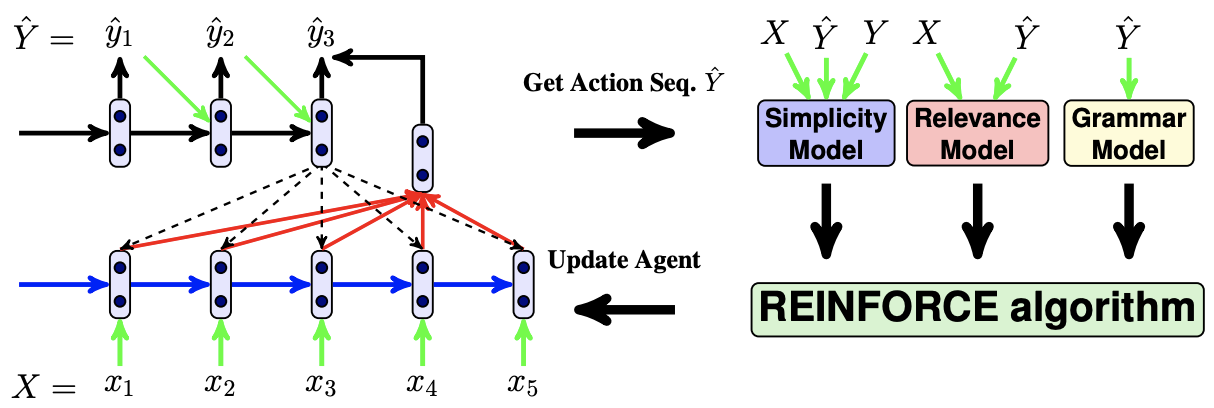
\includegraphics[width=14cm]{Images/dress.png}
    \caption{DRESS model. \textit{X} is the complex sentence, \textit{Y} is the reference sentence and \textit{$\hat{Y}$} simplification produced by the encoder-decoder model. Source: \cite{zhang-lapata-2017-sentence}.}
    \label{fig:dress}
\end{figure}

\cite{zhang-lapata-2017-sentence} proposed a \emph{deep reinforcement sentence simplification model} (DRESS, fig. \ref{fig:dress}) with an encoder-decoder architecture implemented by recurrent neural networks (RNNs). To make the output simpler and grammatically correct while also preserving the meaning of the input, they trained the model in a \emph{reinforcement learning} (RL) framework. It explores the space of possible simplifications while learning to maximize an expected reward function that encourages outputs that meets simplification constraints.

\section{Simplification as a style transfer}

Text simplification can be viewed as a form of \emph{style transfer} (\cite{wubben-etal-2012-sentence}; \cite{sulem-semantic-evaluation}), or \emph{stylistic paraphrasing}, with the goal of rewriting a sentence such that we preserve the meaning but alter the style. Generating paraphrases targeting a more general interpretation of style was first attempted in (\cite{xu-etal-2012-paraphrasing}). All of these works are based on statistical machine translation methods. 

Recently, however, the advances in neural machine translation have started to be applied to general stylistic paraphrasing. The Shakespeare dataset (\cite{xu-etal-2012-paraphrasing}) was used recently with a variation of Seq2Seq models (\cite{jhamtani-etal-2017-shakespearizing}). They proposed to use a mixture model of \emph{pointer network} and \emph{Long Short-Term Memory} (LSTM) to transform a modern English text to a Shakespearean style English. The authors reported an improvement over statistical machine translation methods. Another impressive work in this direction uses a large set of Bible translations to transfer a prose style with an encoder-decoder recurrent neural network and \emph{Moses} - a statistical machine translation system (\cite{carlson-bible}). Table \ref{tab:bible-style-transfer} gives some examples produced by this approach. 

\begin{table}[h]
\centering
\begin{tabular}{p{3.1cm}p{3.1cm}p{3.1cm}p{3.1cm}}
\hline
\textbf{Source} & \textbf{Target} & \textbf{Moses output} & \textbf{Seq2Seq} \\
\hline
Then Samuel gave him an account of everything, keeping nothing back. And he said, It is the Lord; let him do what seems good to him. & And Samuel told him every whit, and hid nothing from him. And he said, It is Jehovah: let him do what seemeth him good. & Then Samuel told him of all things not. And he said, It is Jehovah; let him do that which seemeth him good. & And Samuel told all things, and did not hold back. And he
said, It is Jehovah; let him do what seemeth good to him.\\
&&& \\
And Jehovah saith, 'Judah doth go up; lo, I have given the land into his hand'. & And the Lord said, Judah is to go up: see, I have given the land into his hands. & And the Lord said, 'Judah will go up, see, I have given the land into his hand.' & And the Lord said, Judah will go up; see, I will give the land into his hand.\\
\hline
\end{tabular}
\caption{Examples which show Moses and Seq2Seq Bible style transfer. Source: \cite{carlson-bible}.}
\label{tab:bible-style-transfer}
\end{table}

Unfortunately, the lack of appropriate training corpora has complicated the direct application of the style transfer approaches to text simplification.  

\section{Unsupervised style transfer}

In contrast, unsupervised style transfer algorithms work with unlabeled datasets which are significantly cheaper and easier to obtain. However, they are also considerably less explored in the literature. Amongst the few exceptions, are: 

\cite{Paetzold:2016:ULS:3016387.3016433} who proposed an unsupervised lexical simplification technique that replaces complex words in the input with simpler synonyms, which are extracted and disambiguated using word embeddings. 

\cite{Shen:2017:STN:3295222.3295427} who proposed to apply an \emph{adversarial training} to unsupervised style transfer and introduced a refined alignment of sentence representations across text corpora. They build an encoder that takes a sentence and its original style indicator as input and maps it to a style-independent content representation that is passed to a style-dependent decoder. The key contribution of this approach is in applying discriminators both on the encoder representation and on the hidden states of the decoders to ensure that they have the same distribution.

\cite{Zhang2018StyleTA} who proposed a two-stage joint training method to boost source-to-target and target-to-source style transfer systems using non-parallel text. They build bidirectional word-to-word style transfer systems in a statistical machine translation framework to generate a pseudo-parallel corpus and constructed two attention-based neural machine translation style transfer systems with the pseudo corpus. Then an iterative back-translation algorithm was employed to better leverage non-parallel text to jointly improve bidirectional neural machine translation based style transfer models.

\cite{surya-etal-2019-unsupervised} who used unlabeled corpora containing simple and complex sentences to train the system based on the shared encoder and two decoders. They proposed a novel training scheme which allows the model to perform content reduction and lexical simplification simultaneously through proposed losses and de-noising.

In comparison with the above-mentioned unsupervised models, we explore a novel application of the architecture for cross-lingual language modeling to the task of text simplification. Our approach achieves superior BLEU and SARI results on the Wikilarge dataset. In addition, we conduct a more comprehensive evaluation and assess the system's performance from a wider variety of metrics (see Chapter \ref{chap:methodology} and \ref{chap:experiments} for details).


\section{From LSTM to Transformers}
\label{sec:from_lstm_to_transformers}

More generally, the recent trend in natural language processing research has been around using \emph{Transformer} neural network architectures which are based on \emph{attention mechanisms} (\cite{NIPS2017_7181}). Thus, \cite{Radford2018}, \cite{howard-ruder-2018-universal} and \cite{Devlin2019BERTPO} investigated language modeling for pre-training Transformer encoders and demonstrated dramatic improvements on classification tasks from the GLUE benchmark (\cite{wang-etal-2018-glue}). \cite{ramachandran-etal-2017-unsupervised} showed that machine translation tasks can also gain significant improvements by utilizing language modeling pre-training.

\cite{zhao2018integrating} introduced a supervised sentence simplification model based on the Transformer architecture and proposed two approaches to integrating the Simple PPDB (\cite{pavlick-callison-burch-2016-simple}) knowledge base for simplification that contains 4.5 million paraphrase rules. The first one is the \emph{Deep Memory Augmented Sentence Simplification} (DMASS) model. It has an augmented dynamic memory to record multiple key-value pairs for each rule in the Simple PPDB which helps to overcome the problem when the neural network focuses more on frequent rules and ignores rare rules. The second model, \emph{Deep Critic Sentence Simplification} (DCSS), encodes the context and the output of each simplification rules into the shared parameters. 

\cite{Mikolov2013ExploitingSA}, \cite{Faruqui2014ImprovingVS}, \cite{Xing2015NormalizedWE} and \cite{Ammar2016MassivelyMW} investigated usage of small dictionaries to align \emph{word representations} from different languages. The need for cross-lingual supervision was slashed by \cite{DBLP:journals/corr/SmithTHH17} and completely removed by \cite{conneau2017word}.

\bigskip
Numerous works on the text simplification task prove once again its importance. Recent advances in the field of NLP have been dictated by \textit{Transfer Learning} methods with Transformer language models. They became the source of our inspiration for this work and we believe they can rise text simplification systems to a new level.

\endinput 

\chapter{Evaluation}
\label{chap:evaluation}

It is widely accepted that text simplification can be performed by \emph{splitting}, \emph{deletion} and \emph{paraphrasing} (\cite{feng}). The splitting operation breaks down a long
sentence into shorter ones. Deletion gets rid of unimportant parts of a sentence. The paraphrasing operation includes reordering, lexical substitutions and syntactic transformations (\cite{xu-etal-2016-optimizing}). The best method for determining the quality of simplification is through human evaluation. Traditionally, a simplified output is judged in terms of grammaticality, meaning preservation and simplicity. For training and comparing models, the most commonly used automatic metrics are:

\begin{itemize}
    \item \emph{BLEU}, to assess an extent to which the output differs from the references;
    \item \emph{SARI}, to evaluate the quality of the output by comparing it against the input and references;
    \item \emph{FKGL}, to estimate the readability of the output.
\end{itemize}

\section{BLEU}
\label{sec:bleu}

BLEU (\emph{Bilingual Evaluation Understudy}) is a precision-oriented metric that estimates the proportion of \textit{n}-gram matches between a system’s output and a reference (\cite{papineni-etal-2002-bleu}). It was one of the first metrics which had shown a high correlation with human judgments of quality and remains one of the most popular automated, inexpensive and language-independent metrics.

BLEU uses a modified precision to compare a candidate translation against multiple references. The reason for the modification is that machine translation systems can generate more words than there are in the references. A simple precision measure sums the number of candidate \textit{n}-grams which appear in any reference and then divides it by the total number of \textit{n}-grams in the candidate translation. This may result in a poor translation with high precision (Table \ref{tab:poor-translation}).

\begin{table}[h]
\centering
\begin{tabular}{ll}
\hline
Candidate: & {\fontfamily{pcr}\selectfont the the the the the the the.} \\
Reference 1: & {\fontfamily{pcr}\selectfont The cat is on the mat.} \\
Reference 2: & {\fontfamily{pcr}\selectfont There is a cat on the mat.} \\
\hline
\end{tabular}
\caption{Example of poor machine translation output with high precision. Source: \cite{papineni-etal-2002-bleu}.}
\label{tab:poor-translation}
\end{table}

\bigskip
All seven words in the candidate translation appear in the references. Thus a unigram simple precision is:

\[P=\frac{m}{w_t}=\frac{7}{7}=1\]

where $m$ is a number of words from the candidate found in the references, and $w_{t}$ is the total number of words in the candidate. This is an example of a perfect score given for a poor translation.

A simple modification solves this issue. To calculate modified unigram precision we first count the maximum number of times a word occurs in any single reference translation. Next, we clip the total count of each candidate word by its maximum
reference count $Count_{clip} = min(Count, Max\_Ref\_Count)$, add these clipped counts up, and divide by the total (unclipped) number of candidate words (\cite{papineni-etal-2002-bleu}). In the above example, the modified unigram precision score would be:

\[P=\frac{min(Count, Max\_Ref\_Count)}{w_t}=\frac{min(7, 2)}{7}=\frac{2}{7}\]

The modified \textit{n}-gram precision is computed similarly for any \textit{n}: all candidate \textit{n}-gram counts and their corresponding maximum reference counts are collected. The candidate counts are clipped by their corresponding reference maximum value, summed, and divided by the total number of candidate \textit{n}-gram. The \textit{n} which has the highest correlation with human judgments was found to be 4. The unigram scores account for the adequacy of the translation, while the longer \textit{n}-gram account for the fluency (\cite{papineni-etal-2002-bleu}).

One of the problem with the modified \textit{n}-gram precision is that it fails to enforce the proper translation length. A possible candidate translation for the above example might be {\fontfamily{pcr}\selectfont the cat} and the modified unigram precision would be:

\[P=\frac{1}{2} + \frac{1}{2}=1\]

To overcome this problem a \emph{multiplicative brevity penalty factor} is used. With the brevity penalty in place, a high-scoring candidate translation must match the reference translations in length, in word choice, and in word order (\cite{papineni-etal-2002-bleu}). If the total length of the translation corpus $c$ is less then or equal to the total length of the reference corpus $r$, the brevity penalty is decaying exponential with $r/c$: 

\[BP=e^{1-\frac{r}{c}}\]

Thus BLEU score is the geometric mean of the test corpus’s modified precision scores multiplied by an exponential brevity penalty factor. Geometric average of the modified \textit{n}-gram precisions, $p_{n}$, is calculated using \textit{n}-grams up to $N$ and positive weights $w_{n}$ summing to 1:

\[BLEU=BP \times \exp(\sum_{n=1}^{N}w_n \log p_n)\]

Despite being widely used and considered to be an informative metric for text-to-text generation, including text simplification, BLEU is not well suited for assessing simplicity from a lexical point of view (\cite{xu-etal-2016-optimizing}). Moreover, BLEU often negatively correlates with simplicity, essentially penalizing simpler sentences (\cite{sulem-etal-2018-bleu}).

\section{SARI}

\emph{SARI}, introduced by \cite{xu-etal-2016-optimizing}, compares system output against the references and against the input sentence. It measures how the simplicity of a sentence was improved based on the words added, deleted and kept by the system (fig. \ref{fig:sari}).

\begin{figure}[h]
    \centering
    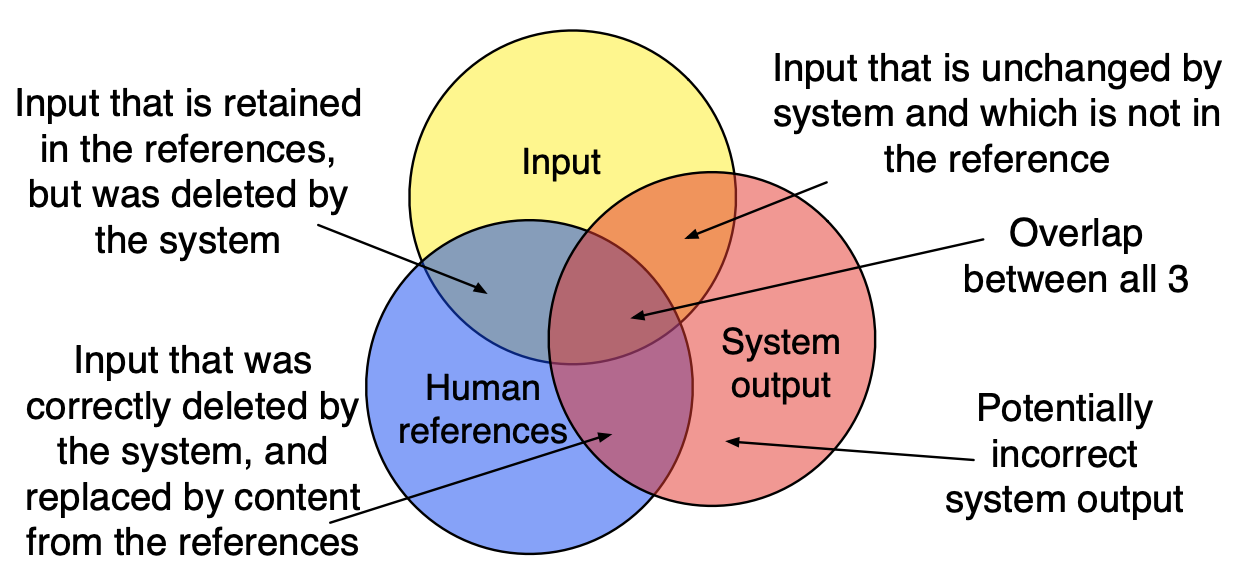
\includegraphics[width=10cm]{Images/sari.png}
    \caption{Metrics that evaluate the output of monolingual text-to-text generation systems. The different regions of this Venn diagram are treated differently with the SARI metric. Source: \cite{xu-etal-2016-optimizing}.}
    \label{fig:sari}
\end{figure}

\bigskip
SARI rewards addition operations, where system output $O$ was not in the input $I$ but occurred in any of the references $R$, i.e. $O\cap \bar{I} \cap R$. We define \textit{n}-gram precision $p(n)$ and recall $r(n)$ for addition operations as follows (\cite{xu-etal-2016-optimizing}):

\begin{equation}
p_{add}(n)=\frac{\sum_{g \in O} \min \left(\#_{g}(O \cap \bar{I}), \#_{g}(R)\right)}{\sum_{g \in O} \#_{g}(O \cap \bar{I})} 
\end{equation}

\begin{equation}
r_{add}(n) =\frac{\sum_{g \in O} \min \left(\#_{g}(O \cap \bar{I}), \#_{g}(R)\right)}{\sum_{g \in O} \#_{g}(R \cap \bar{I})} 
\end{equation}

where $\#g(\cdot)$ is a binary indicator of occurrence of \textit{n}-grams $g$ in a given set and

\setlength\extrarowheight{10pt}
\hspace*{3em}
\begin{tabular}{l}
$\#_{g}(O \cap \bar{I})=\max \left(\#_{g}(O)-\#_{g}(I), 0\right)$ \\
$\#_{g}(R \cap \bar{I})=\max \left(\#_{g}(R)-\#_{g}(I), 0\right)$
\end{tabular}

\bigskip
Example below (Table \ref{tab:sari-example}) demonstrates how the addition of word \textit{now} is rewarded in both $p_{add}(n)$ and $r_{add}(n)$, but the addition of \textit{you} in \textit{Output 1} is penalized in $p_{add}(n)$.

\setlength\extrarowheight{0pt}
\begin{table}[h]
\centering
\begin{tabular}{ll}
\hline
Input: & {\fontfamily{pcr}\selectfont About 95 species are currently accepted.} \\
Reference 1: & {\fontfamily{pcr}\selectfont About 95 species are currently known.} \\
Reference 2: & {\fontfamily{pcr}\selectfont About 95 species are now accepted.} \\
Reference 3: & {\fontfamily{pcr}\selectfont 95 species are now accepted.} \\
Output 1: & {\fontfamily{pcr}\selectfont About 95 you now get in.} \\
Output 2: & {\fontfamily{pcr}\selectfont About 95 species are now agreed.} \\
Output 3: & {\fontfamily{pcr}\selectfont  About 95 species are currently agreed.} \\
\hline
\end{tabular}
\caption{Example of sentence simplifications for SARI calculation. Source: \cite{xu-etal-2016-optimizing}.}
\label{tab:sari-example}
\end{table}

\bigskip
The $SARI$ scores for these outputs are $0.2683$, $0.7594$, and $0.5890$ respectively. The BLEU scores are $0.1562$, $0.6435$, and $0.6435$. BLEU is unable to separate \textit{Output 2} and \textit{Output 3} because matching any of the references is rewarded in the same way.

SARI rewards keep operation, where \textit{n}-grams are retained in both output and references. Number of such references matters. It bears in mind that some words or phrases don't require simplification:

\begin{equation}
p_{keep}(n)=\frac{\sum_{g \in I} \min \left(\#_{g}(I \cap O), \#_{g}I \cap R')\right)}{\sum_{g \in I} \#_{g}(I \cap O)} 
\end{equation}

\begin{equation}
r_{keep}(n) =\frac{\sum_{g \in I} \min \left(\#_{g}(I \cap O), \#_{g}(I \cap R')\right)}{\sum_{g \in I} \#_{g}(I \cap R')} 
\end{equation}

where

\setlength\extrarowheight{10pt}
\hspace*{3em}
\begin{tabular}{l}
$\#_{g}(I \cap O)=\min \left(\#_{g}(I), \#_{g}(O)\right)$ \\
$\#_{g}(I \cap R')=\min \left(\#_{g}(I), \#_{g}(R)/r\right)$
\end{tabular}

\bigskip
$R'$ indicates the \textit{n}-gram count over $R$ with fractions. In the above example (Table \ref{tab:sari-example}) 2 out of the total $r=3$ references contain the word {\fontfamily{pcr}\selectfont  about}, thus its count is weighted by 2/3.

For deletion, SARI calculates precision only. Deleting too many words decreases readability far more than not deleting:

\begin{equation}
p_{del}(n)=\frac{\sum_{g \in I} \min \left(\#_{g}(I \cap \bar{O}), \#_{g}I \cap \bar{R'})\right)}{\sum_{g \in I} \#_{g}(I \cap \bar{O})} 
\end{equation}

where

\setlength\extrarowheight{10pt}
\hspace*{3em}
\begin{tabular}{l}
$\#_{g}(I \cap \bar{O})=\max \left(\#_{g}(I) - \#_{g}(O), 0\right) $ \\
$\#_{g}(I \cap \bar{R'})=\max \left(\#_{g}(I) - \#_{g}(R)/r, 0\right)$
\end{tabular}

\bigskip
Final SARI score calculates arithmetic average of \textit{n}-gram precisions and recalls:

\begin{equation}
SARI=d_{1} F_{add}+d_{2} F_{keep}+d_{3} P_{del}
\end{equation}

where 

\setlength\extrarowheight{12pt}
\hspace*{3em}
\begin{tabular}{l}
$d_{1}=d_{2}=d_{3}=1/3$ \\
$P_{operation}=\frac{1}{k} \sum_{n=[1, \ldots, k]} p_{operation}(n)$ \\
$R_{operation}=\frac{1}{k} \sum_{n=[1, \ldots, k]} r_{operation}(n)$ \\
$F_{operation}=\frac{2 \times P_{operation} \times R_{operation}}{P_{operation}+R_{operation}}$ \\
$operation \in[del, keep,add]$
\end{tabular}
\setlength\extrarowheight{0pt}

\bigskip
where $k$ is the highest \textit{n}-gram order.

\section{BLEU vs SARI}

\cite{xu-etal-2016-optimizing} and \cite{wubben-etal-2012-sentence} showed that $BLEU$ does not demonstrate significant correlation with the simplicity scores rated by humans. In contrast, SARI achieves a much better correlation with human evaluations of simplicity. On the other hand, BLEU has a higher correlation on grammaticality and meaning preservation. BLEU gives a higher score to an output that is not too short and contains only \textit{n}-grams that occur in references. When applied to monolingual tasks like simplification, it does not take into account any differences between the input and the references. Whereas SARI considers both precision and recall looking at the differences between the references and the input (\cite{xu-etal-2016-optimizing}).

\begin{figure}[h]
    \centering
    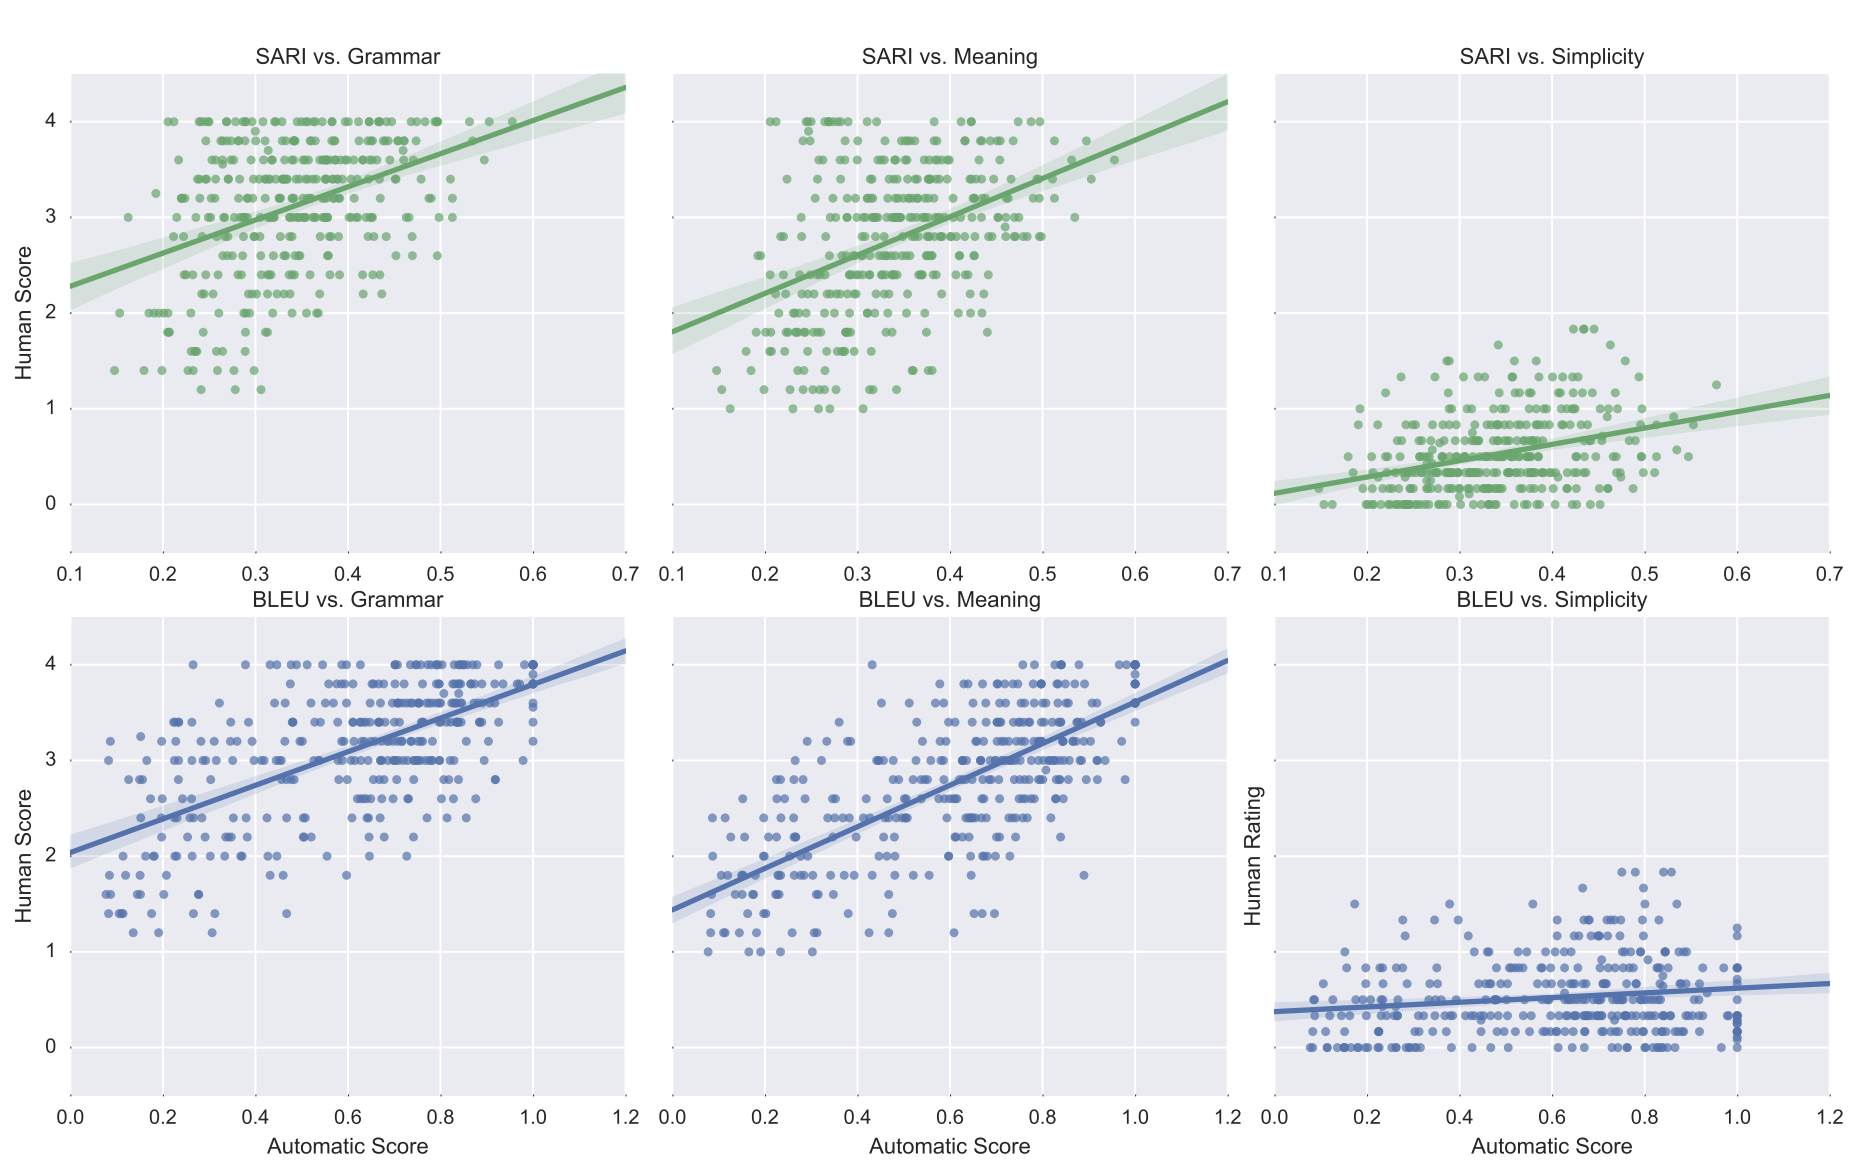
\includegraphics[width=14cm]{Images/bleu-sari.png}
    \caption{Scatter plots of automatic metrics against human scores for individual sentences. Source: \cite{xu-etal-2016-optimizing}.}
    \label{fig:bleu-sari}
\end{figure}

\bigskip
Scatter plots in fig. \ref{fig:bleu-sari} highlights the correlation of human scores on meaning and grammar with BLEU and on simplicity with SARI. The outputs which are similar to the input get a high BLEU score. That is because for the monolingual simplification task, the more references are created the more \textit{n}-grams of the input are included in the references. Outputs with few changes receive high grammar and meaning scores from humans as well, but it does not imply that they are good simplifications. Thus, BLEU prefers conservative systems that make few or no changes, while SARI penalizes them.

\section{FKGL}

Flesch-Kincaid Grade Level (FKGL) estimates the readability of text using cognitively motivated features (\cite{Kincaid1975DerivationON}). A lower value indicating higher readability. Commonly reported as measures of simplicity, FKGL relies on average sentence lengths and the number of syllables per word. Short sentences get low scores even if they have poor grammaticality or do not preserve meaning (\cite{wubben-etal-2012-sentence}). FKGL was developed by J. Peter Kincaid for the U.S. Navy in 1975. The Navy used the Flesch-Kincaid Grade score for assessing the difficulty of technical manuals.

The grade level is calculated with the following formula:

\begin{equation}
0.39\left(\frac{\#words}{\#sentences}\right)+11.8\left(\frac{\#syllables}{\#words}\right)-15.59
\end{equation}

\bigskip
A result is a number that corresponds to a US grade level. An FKGL score of 8 means that the reader needs at least a grade 8 level of reading to understand it. The FKGL coefficients were derived via multiple regressions applied to the reading compression test scores of 531 Navy personnel reading training manuals (\cite{xu-etal-2016-optimizing}). The more words a sentence contains the more difficult it is. Similarly, words with many syllables are harder to read than words that use fewer.

\section{Automatic sentence simplification evaluation}
\label{sec:easse}

\cite{alva-manchego-etal-2019-easse} introduced the \emph{Easier Automatic Sentence Simplification Evaluation} (EASSE) framework\footnote{\href{https://github.com/feralvam/easse}{https://github.com/feralvam/easse}}, a Python package for automatic evaluation of the sentence simplification. EASSE provides a broad range of evaluation resources from standard automatic metrics (e.g. BLEU, SARI, FKGL) to quality estimations and comprehensive HTML reports on quantitative and qualitative assessments of a  simplification output.

Using both the source sentence and the output simplification quality estimation, it brings additional insights into simplification systems which are not revealed by automatic metrics, e.g.: 

\begin{itemize}
    \item \emph{compression ratio}, the length of the output sentence divided by the length of the input sentence;
    \item \emph{proportion of exact matches} with the original sentences;
    \item average \emph{proportion of added words};
    \item average \emph{proportion of deleted words}.
\end{itemize}

\bigskip
In this section, we found out that the evaluation of text simplification is not a simple task and requires multiple metrics for an accurate assessment. In this work, we will use BLEU, SARI, FKGL, Exact matches ratio, Addition, and Deletion ratios. In addition, in Section \ref{sec:training-details} we introduce \textit{Compound Simplification Score} for comparing models with different BLEU, SARI and FKGL scores.


\endinput
\chapter{Datasets description}
\label{chap:datasets}

We conducted our experiments on three different simplification datasets, the summary statistics of which are presented in Table \ref{tab:datasets}.

\begin{table}[h]
\centering
\begin{tabular}{m{5cm}ccc}
\hline
\textbf{} & \textbf{WikiLarge} & \textbf{Newsela} & \textbf{News Crawl/SW-CBT} \\
\hline
Source (monolingual) & 291,402 & 81,705 & 1,500,000 \\
Target (monolingual) & 291,402 & 76,073 & 1,489,778 \\
Train set & 5,000 & 5,000 & - \\
Validation set & 2,000 & 1,500 & - \\
Test set & 359 & 1,500 & - \\
Vocab source  & 41,303 & 33,316 & 43,222 \\
Vocab target & 39,912 & 22,405 & 49,118 \\
Compression ratio & 0.98 & 0.76 & 1.21 \\
Sentence splits & 1.09 & 1.01 & 0.99 \\
FKGKL (source) & 9.51 & 8.51 & 7.89 \\
FKGKL (target) & 6.33 & 2.86 & 5.46 \\
\hline
\end{tabular}
\caption{Datasets.}
\label{tab:datasets}
\end{table}

\section{WikiLarge}

The \emph{Parallel Wikipedia Simplification} (PWKP) corpus introduced by \cite{zhu-etal-2010-monolingual} has become a benchmark for training and evaluating text simplification models. It constitutes a collection of parallel sentences from the English Wikipedia\footnote{\href{https://en.wikipedia.org/}{https://en.wikipedia.org/}} and Simple English Wikipedia\footnote{\href{https://simple.wikipedia.org/}{https://simple.wikipedia.org/}}. Simple English Wikipedia is an online encyclopedia aimed at children and adults who are learning the English language. Its articles contain fewer words and simpler grammar than those in English Wikipedia.

WikiLarge is a Wikipedia corpus constructed by \cite{zhang-lapata-2017-sentence}. It is a combination of three datasets:

\begin{itemize}
    \item PWKP (\cite{zhu-etal-2010-monolingual}), the dataset described above;
    \item aligned sentence pairs from \cite{Kauchak2013ImprovingTS};
    \item aligned and revisioned sentence pairs from \cite{Woodsend2011LearningTS}.
\end{itemize}

Originally it had 296,402 sentence pairs but we took 5,000 pairs for machine translation step during our model training (see Chapter \ref{chap:experiments} for details). For validations and tests, we used datasets created by \cite{xu-etal-2016-optimizing}. They consist of complex sentences from the WikiSmall dataset aligned with simplifications provided by \emph{Amazon Mechanical Turk}~\footnote{\href{https://www.mturk.com/}{https://www.mturk.com/}}. Each original sentence in the dataset has 8 simplified references. See Table \ref{tab:datasets} for details.

\section{Newsela}
\label{sec:newsela-dataset}

\emph{Newsela} dataset was introduced by \cite{xu-etal-2015-problems}. The authors argued that Wikipedia as a simplification data resource is sub-optimal because it is prone to automatic sentence alignment errors, contains a large proportion of inadequate simplifications and it generalizes poorly to other text genres.

Newsela is a platform that provides reading materials for classroom usage\footnote{\href{https://newsela.com/}{https://newsela.com/}}. On request, they provide a corpus that includes thousands of news articles professionally leveled to different reading complexities. For every original sentence (Version 0) there are 4 or 5 simplified versions (Version 5 or 6 being the simplest).

We used the most contrast article versions: 0-level for a source dataset and 4-level for a target dataset. For the machine translation step, for the test, and for the validation datasets we used parallel complex-simple pairs provided by \cite{xu-etal-2015-problems}. See Table \ref{tab:datasets} for details.

\section{News Crawl and SimpleWiki with Children's Books Test}
\label{dataset:sw-cbt}

To test the performance of our model on a corpus of different styles and sizes we collected our own datasets for training and used the Wikilarge and the Newsela sets for the machine translation step, test and validation.

As a source "complex" monolingual dataset we used 1,500,000 sentences from the WMT 2014 News Crawl\footnote{\href{http://statmt.org/wmt14/training-monolingual-news-crawl/}{http://statmt.org/wmt14/training-monolingual-news-crawl/}}, a dataset consisting of text crawled from online news. For target "simple" dataset we combined sentences from SimpleWiki (SW)\footnote{\href{https://dumps.wikimedia.org/simplewiki/latest/}{https://dumps.wikimedia.org/simplewiki/latest/}} with the Children's Books Test (CBT) from \cite{Hill2015TheGP}. The CBT is built from children books freely provided by Project Gutenberg \footnote{\href{https://gutenberg.org/}{https://gutenberg.org/}}. After removing duplicates from the SW-CBT dataset, the resulting target monolingual dataset contains 1,489,778 sentences. See Table \ref{tab:datasets} for details.


\section{Data Pre-processing}

For data pre-processing we used a script provided by XLM model\footnote{\href{https://github.com/facebookresearch/XLM/blob/master/get-data-nmt.sh}{https://github.com/facebookresearch/XLM/blob/master/get-data-nmt.sh}}. It uses Moses\footnote{\href{http://www.statmt.org/moses/}{http://www.statmt.org/moses/}} to replaces Unicode punctuation, normalize it, remove non-printing characters and tokenize the data. Then it uses fastBPE\footnote{\href{https://github.com/glample/fastBPE}{https://github.com/glample/fastBPE}} to apply 60,000 BPE (Byte Pair Encoding) codes\footnote{\href{https://dl.fbaipublicfiles.com/XLM/codes_enfr}{https://dl.fbaipublicfiles.com/XLM/codes\_enfr}} to monolingual and parallel test data. These BPE codes were learned during the training of the pre-trained XLM model which we use for our experiments. Finally, the script generates the same shared vocabulary through the BPE codes to improve the alignment of embedding spaces across languages.

\bigskip
In this chapter, we described Wikilarge and Newsela datasets which became benchmarks for the evaluation of text simplification systems. Furthermore, we introduced our own monolingual dataset based on News Crawl, SimpleWiki and Children Books Test. Vocabulary size, compression ratio, and FKGL score prove once again the high quality of the Newsela dataset.

\endinput 
\chapter{Methodology}
\label{chap:methodology}

In this chapter, we outline the methodology for our experiments. First of all, we describe the model we use. Then we review beam search generation and proposed penalization. In the end, we introduce the cross-validation technique we use and reveal details on the training process.

\section{Unsupervised Machine Translation}
\label{sec:xlm}

\cite{lample2017unsupervised} and \cite{artetxe2018iclr} have proposed unsupervised Machine Translation (MT) which relies on monolingual (i.e., non parallel) corpora only. The authors have defined four key principles required for training such models: 

\begin{itemize}
    \item MT system initialization;
    \item language modeling;
    \item iterative back-translation (\cite{sennrich-etal-2016-improving});
    \item shared encoder latent representations.
\end{itemize}

Building on this idea, \cite{lample2018phrase} introduced an UnsupervisedMT\footnote{\href{https://github.com/facebookresearch/UnsupervisedMT}{https://github.com/facebookresearch/UnsupervisedMT}} model that outperforms previous approaches and is easier to train and tune.

\begin{figure}[h]
    \centering
    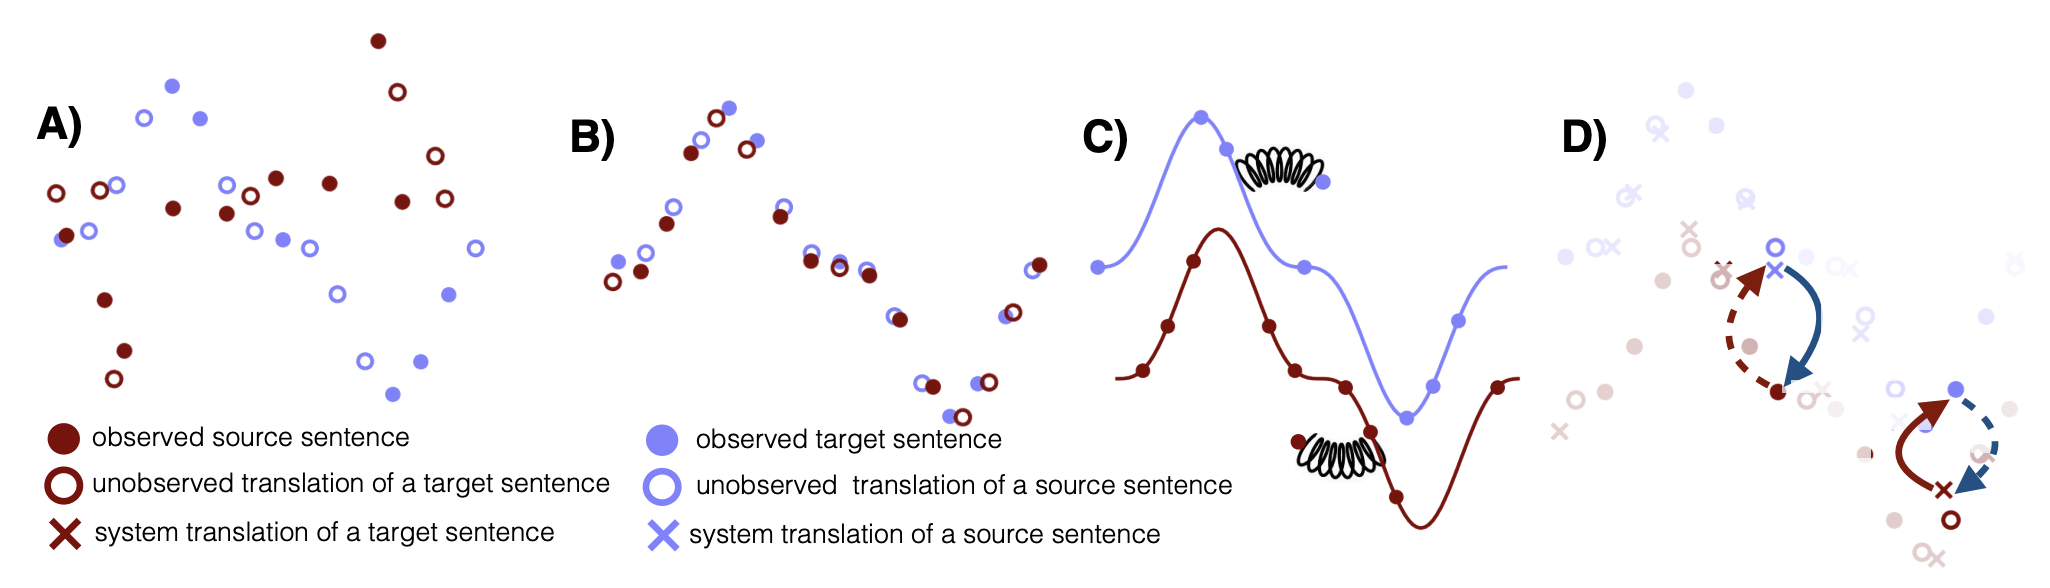
\includegraphics[width=14cm]{Images/unsupervisedNMT.png}
    \caption{Toy illustration of the three principles of unsupervised MT. Source: \cite{lample2018phrase}}
    \label{fig:unsupervisedNMT}
\end{figure}

Fig. \ref{fig:unsupervisedNMT} demonstrates the usage of the above-mentioned principals. A) There are two monolingual corpora. B) \textbf{Initialization}. The two distributions are aligned by performing word-by-word translation. C) \textbf{Language modeling}. A language model is learned independently in each domain to infer the structure in the data. D) \textbf{Back-translation}. Starting from an observed source sentence they use the current source $\rightarrow$ target model(dashed arrow), yielding a potentially incorrect translation (blue cross near the empty circle). Starting from this (back) translation, they use the target $\rightarrow$ source model (continuous arrow) to reconstruct the sentence in the original language. The discrepancy between the reconstruction and the initial sentence provides an error signal to train the target $\rightarrow$ source model parameters. The same procedure is applied in the opposite direction to train the source $\rightarrow$ target model (\cite{lample2018phrase}).

\section{XLM}
\label{sec:xlm}

Based on the ideas of aligning the distributions of sentences in different languages, \cite{lample2019cross} reduced the need for parallel data. They introduced supervised and unsupervised approaches for cross-lingual language models (XLMs\footnote{\href{https://github.com/facebookresearch/XLM}{https://github.com/facebookresearch/XLM}}) training based on Transformers' architecture~\cite{NIPS2017_7181}. The unsupervised method relies on monolingual corpora only, whereas the supervised one leverages parallel data. The XLM model achieves a better performance than the original BERT\footnote{\href{https://github.com/google-research/bert}{https://github.com/google-research/bert}} on all GLUE tasks\footnote{\href{https://github.com/facebookresearch/XLM\#i-monolingual-language-model-pretraining-bert}{https://github.com/facebookresearch/XLM\#i-monolingual-language-model-pretraining-bert}}.

\begin{figure}[h]
    \centering
    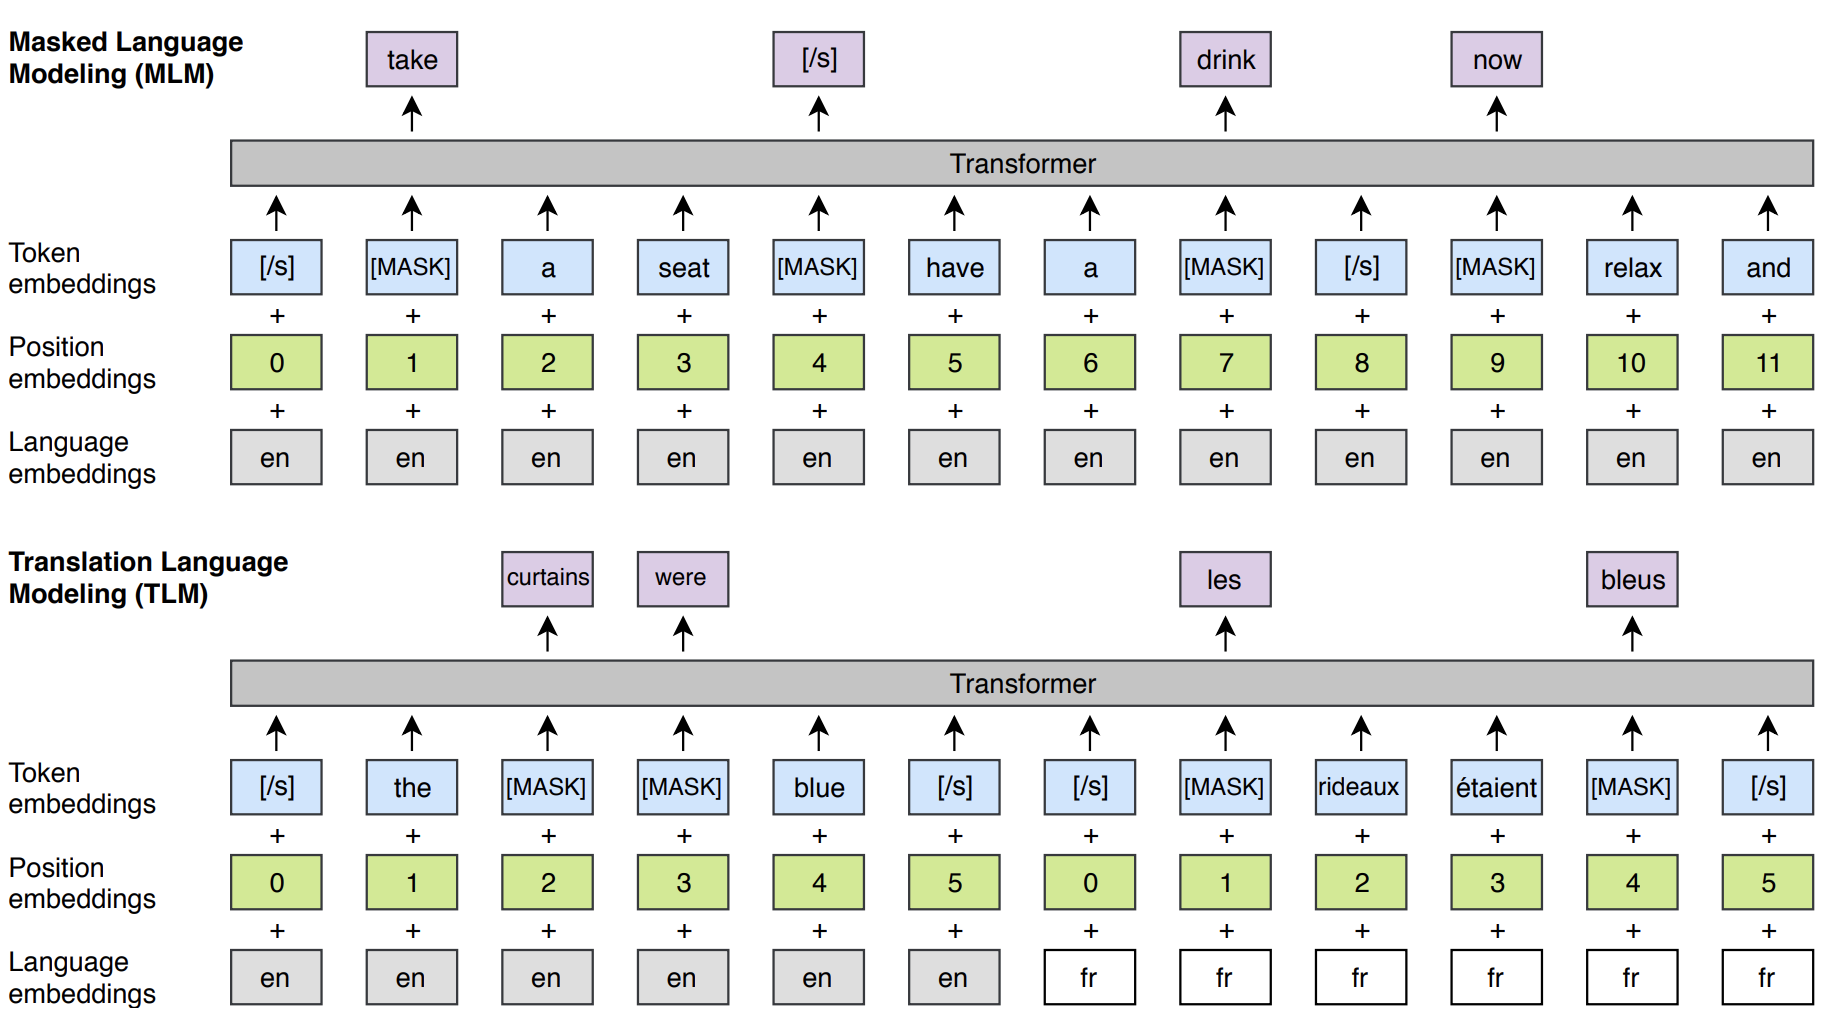
\includegraphics[width=14cm]{Images/xlm.png}
    \caption{Cross-lingual language model pretraining. Source: \cite{lample2019cross}}
    \label{fig:xlm}
\end{figure}

The unsupervised \textbf{cross-lingual text representations} are obtained with the help of \emph{Causal Language Modeling} (CLM) and \emph{Masked Language Modeling} (MLM) training objectives. During training, they process all languages with the same shared vocabulary created through Byte Pair Encoding (BPE) (\cite{Sennrich2015NeuralMT}). CLM is a Transformer language model trained to predict the probability of a word given the previous words in a sentence $P(w_{t}|w_{1}, \dots, {w_{t-1}, \Theta})$. MLM assumes random sampling of 15\% of the BPE tokens from the text streams, replacing them by a [MASK] token 80\% of the time, by a random token 10\% of the time, and keeping them unchanged 10\% of the time (fig. \ref{fig:xlm}). 

Since both the CLM and MLM only require monolingual data, they cannot be used to utilize parallel data. \emph{Translation Language Modeling} (TLM) leverages parallel corpora to improve cross-lingual pre-training. It extends the BERT MLM approach by using parallel sentences (fig. \ref{fig:xlm}). TLM randomly masks words in both the source and target sentences. To predict a word masked in a source sentence, the model can either attend to surrounding source words or to the target translation, encouraging the model to align the source and target representations. The target context can be used if the source one is not sufficient to guess the masked source words (\cite{lample2019cross}).

To the best of our knowledge, cross-lingual language modeling has not been applied before for the task of text simplification. Following this approach, we used the XLM model for our experiments.

We included the following 6 steps into the model training: CLM, TLM, \emph{Parallel Classification} (PC), \emph{Denoising Auto-Encoder} (AE), \emph{Machine Translation} (MT) and \emph{Back-translation} (BT). During the PC step, the model predicts if pairs of sentences are mutual translations of each other. AE and MT steps are similar with the only difference that for AE step the model uses mono language sentences and add noise before masking and encoding. The BT step, described in the previous section, is similar to \cite{lample2018phrase}. MT is a supervised machine translation step. In our experiments, we first consider the settings with no supervision (i.e., by excluding MT and TLM steps) and later added an MT step trained on a small parallel corpus to attest the extent to which a little supervision can help with the simplification problem. It is worth noting that the addition of TLM step, which also relies on parallel corpora, had marginal impact on the performance of the models.   

The importance of each step can be weighted by a coefficient but we did not see any improvement when changing the values of the coefficients and used the default lambdas of 1 for every step.

\section{Beam Search Generation}

Beam Search is a common technique to improve decoding performance. Instead of decoding the most probable words in a greedy fashion, it generates an output sentence by keeping a fixed number (specified by beam size parameter) of hypotheses with the highest log-probability at each step. The approach explores a set of candidate hypotheses until the sentence is fully decoded and selects the one with the highest log-probability at the end (Fig. \ref{fig:beam-search}).

\begin{figure}
    \centering
    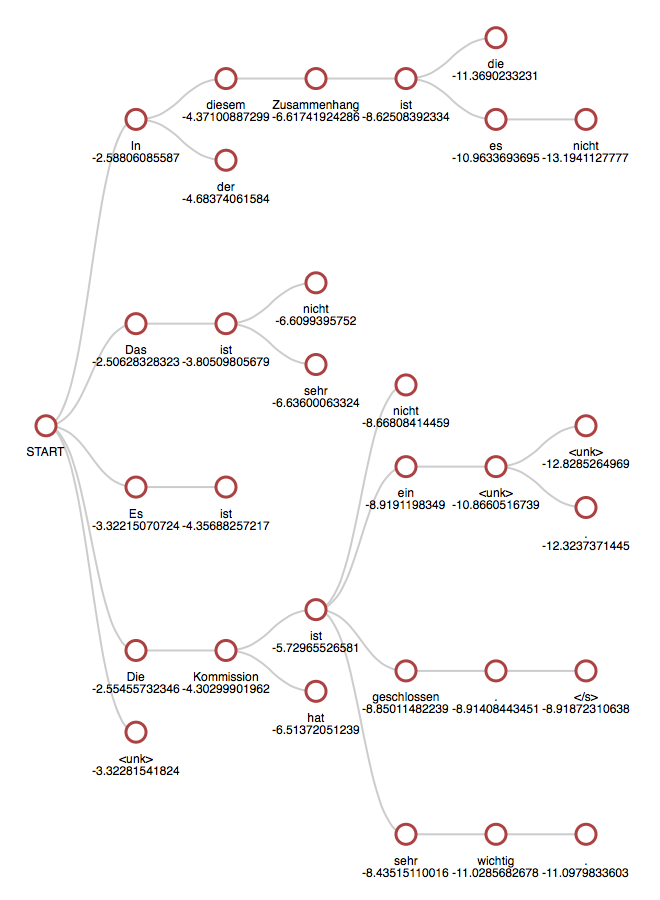
\includegraphics[width=14cm]{Images/beam_search.png}
    \caption{Visualisation of beam search of width 5. Source: OpenNMT.}
    \label{fig:beam-search}
\end{figure}

Such a decoding strategy based on scoring provides us with additional control over sentence generation. To manage the exact matches ratio, length and simplicity (FKGL-based) of a hypothesis we added three types of score penalties. 

\textbf{Length penalty} (LP) favors shorter or longer hypothesis depending on $\lambda_{length}$ parameter:
\medskip
\[LP = \lambda_{length} \times \exp(length(hypothesis))\]
\medskip

\textbf{Exact matches penalty} (EMP) uses cosine similarity between input and hypothesis to restrict copying of input:
\medskip
\[EMP = \lambda_{exact\_matches} \times \exp(cosine\_similarity(input, hypothesis))\]
\medskip

\textbf{FKGL penalty} (FKGLP) encourages hypothesis with lower FKGL score:
\medskip
\[FKGLP = \lambda_{FKGL} \times \exp(FKGL(hypothesis))\]
\medskip

We demonstrate that together these beam search penalties make it possible to improve the decoding results of a model after training.

\section{Random Subsampling Validation}

We choose random sub-sampling validation (\cite{Dubitzky}) for assessing how our models will generalize to an independent data set and for eliminating statistical errors due to dataset split. This approach belongs to \emph{non-exhaustive cross validation} methods. It does not compute all possible splits of the dataset but creates multiple random splits into training and test data (Fig. \ref{fig:subsampling}). For each such split, we train a model on training data and evaluate using test data. The final results are then averaged over the splits. The advantage of this method is that the proportion of the train/test split is not dependent on the number of partitions. The disadvantage is that test sets may overlap and some examples may never be selected. To overcome this possible problem we repeat this procedure 10 times.

\begin{figure}
    \centering
    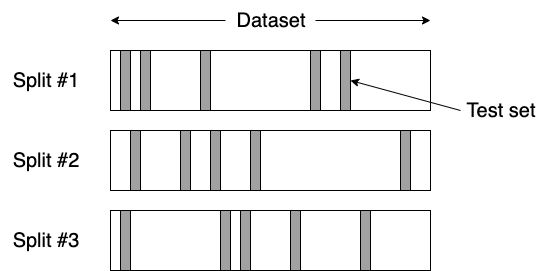
\includegraphics[width=12cm]{Images/subsampling.png}
    \caption{Repeated random subsampling. Grey areas are test data and white ares are train data.}
    \label{fig:subsampling}
\end{figure}


\section{Training Details}
\label{sec:training-details}

We trained our models on the Nvidia Tesla V100 GPU card and used the same hyper-parameters across datasets except for beam search penalty coefficients. 

Both encoder and decoder have \textbf{embedding layer of size 1024}, \textbf{6 attention layers} with \textbf{8 heads} and \textit{GELU} activation function, and regularized with an \textbf{attention dropout rate of 0.1}. 

We used \textit{Adam} optimizer with learning rate decay based on the inverse square root of the update number. \textbf{Learning rate} was set to \textbf{0.0001}, the first momentum coefficient was set to 0.9 and the second momentum coefficient to 0.98.

We examined our XLM models performance based on a range of simplification metrics discussed in Chapter \ref{chap:evaluation}. To determine which set of scores is better we introduced a new \emph{Compound Simplification Score} (CSS). Since BLEU and SARI take values from 0 to 100 (the higher the better) and FKGL takes values from 0 to 10 on our datasets (the lower the better) we defined it as follows:
\[CSS=\frac{BLEU}{100} + \frac{SARI}{100} + \frac{100 - FKGL \times 10}{100}\]

We used CSS as our stopping criteria, i.e., 5 epochs of non-increasing number. We used different epoch sizes for different datasets based on their sizes: 80,000 sentences for Newsela, 150,000 for Wikilarge and 200,000 for News/SW-CBT datasets. On average a single epoch took 15 minutes on Newsela, 35 minutes on Wikilarge and 40 minutes on News/SW-CBT datasets. All our models on all the datasets converged within 10-15 epochs.

\endinput
\chapter{Experiments}
\label{chap:experiments}

We performed our experiments on the XLM model described in Section \ref{sec:xlm}. The baseline unsupervised XLM models trained on Newsela and Wikilarge datasets gave us encouraging results in comparison with the supervised models from the literature. Further improvements achieved by adding limited supervised Machine translation (MT) step, new monolingual corpora and modified beam search generation led us to the best SARI result on Newsela dataset and the best BLEU result on Wikilarge dataset. 


\section{Comparison models}

We compared the performance of our model against multiple others mentioned in Chapter \ref{chap:related_works}. \emph{PBMT-R} is phrase-based machine translation system with a re-ranking post-processing step proposed by \cite{wubben-etal-2012-sentence}. \emph{Hybrid} is a simplification model that includes a probabilistic model for splitting and dropping and a PBMT-R model for substitution and reordering (\cite{narayan-gardent-2014-hybrid}). \emph{SBMT-SARI} is a syntax-based translation model trained on PPDB (\cite{ganitkevitch-etal-2013-ppdb}) and trained with SARI (\cite{zhang-lapata-2017-sentence}). \emph{EncDecA}, a basic attention-based encoder-decoder model, \emph{DRESS}, a deep reinforcement learning model, \emph{DRESS-LS}, a linear combination of DRESS and the lexical simplification model, all of them were introduced in \cite{zhang-lapata-2017-sentence}. \emph{DMASS+DCSS} is a combination of DMASS and DCSS models from \cite{zhao2018integrating} (Section \ref{sec:from_lstm_to_transformers}).

The BLEU, SARI and FKGL results for the above-mentioned models were taken from \cite{zhang-lapata-2017-sentence} and \cite{zhao2018integrating}. For the models introduced in Chapter \ref{chap:methodology} we also report Exact matches, Addition and Deletion ratios which provide additional insights into performance of simplification systems.

\begin{table}
\centering
\begin{tabular}{m{4.5cm}cccccc}
\hline
\textbf{} & \textbf{BLEU} & \textbf{SARI} & \textbf{FKGL} & \textbf{Exact Match} & \textbf{Add.} & \textbf{Del.} \\
\hline
PBMT-R & 18.19 & 15.77 & 7.59 & - & - & - \\
Hybrid & 14.46 & 30.00 & 4.01 & - & - & - \\
EncDecA & 21.7.0 & 24.12 & 5.11 & - & - & - \\
DRESS & 23.21 & 27.37 & 4.13 & - \\
DRESS-LS & \textbf{24.30} & 26.63 & 4.21 & - & - & - \\
DMASS+DCSS  & - & 27.28 & 5.17 & - & - & - \\
XLM & 16.97 & 19.32 & 10.52 & 0.46 & 0.04 & 0.05 \\
XLM (News/SW-CBT) & 18.50 & 12.94 & 10.36 & 0.97 & 0.00 & 0.00 \\
XLM (News/SW-CBT, penalized beam) & 18.34 & 13.49 & 8.46 & 0.72 & 0.01 & 0.00 \\
XLM (MT) & 19.44 & \textbf{43.18} & 4.18 & 0.09 & 0.12 & 0.53 \\
XLM (MT, News/SW-CBT) & 19.33 & 39.60 & 5.57 & 0.21 & 0.10 & 0.45 \\
XLM (MT, News/SW-CBT, penalized beam) & 16.56 & 42.24 & \textbf{3.58} & 0.04 & 0.1 & 0.6  \\
\hline
Output = Source & 18.52 & 12.78 & 10.36 & 1.00 & 0.00 & 0.00 \\
Output = Target & 100.00 & 100.00 & 4.18 & 0.00 & 0.19 & 0.61 \\
\end{tabular}
\caption{Automatic evaluation on Newsela test set. Source: \cite{zhang-lapata-2017-sentence}, \cite{zhao2018integrating}.}
\label{tab:newsela-results}
\end{table}

\begin{table}
\centering
\begin{tabular}{m{4.5cm}cccccc}
\hline
\textbf{} & \textbf{BLEU} & \textbf{SARI} & \textbf{FKGL} & \textbf{Exact Match} & \textbf{Add.} & \textbf{Del.} \\
\hline
PBMT-R & 81.11 & 38.56 & 8.33 & - & - & - \\
Hybrid & 48.97 & 31.40 & \textbf{4.56} & - & - & - \\
SBMT-SARI & 73.08 & 39.96 & 7.29 & - & - & - \\
EncDecA & 88.85 & 35.66 & 8.41 & - & - & - \\
DRESS & 77.18 & 37.08 & 6.58 & - & - & - \\
DRESS-LS & 80.12 & 37.27 & 6.62 & - & - & - \\
DMASS+DCSS  & - & \textbf{40.42} & 7.18 & - & - & - \\
UNTS+10K & 76.13 & 35.29 & - & - & - & - \\
XLM & 94.83 & 28.30 & 9.75 & 0.76 & 0.02 & 0.01 \\
XLM (News/SW-CBT) & \textbf{96.91} & 28.00 & 9.94 & 0.93 & 0.00 & 0.00 \\
XLM (News/SW-CBT, penalized beam) & 94.95 & 30.03 & 9.82 & 0.45 & 0.01 & 0.03 \\
XLM (MT) & 92.66 & 30.99 & 9.68 & 0.73 & 0.02 & 0.02 \\
XLM (MT, News/SW-CBT) & 96.05 & 29.44 & 9.81 & 0.89 & 0.01 & 0.02 \\
XLM (MT, News/SW-CBT, penalized beam) & 76.93 & 35.63 & 7.74 & 0.3 & 0.04 & 0.26 \\
XLM (MT, Newsela) & 3.63 & 31.80 & 6.24 & 0.01 & 0.17 & 0.44 \\
\hline
Output = Source & 97.41 & 27.32 & 9.90 & 1.00 & 0.00 & 0.00 \\
Output = Target & 68.87 & 40.83 & 8.33 & 0.00 & 0.19 & 0.21 \\
\end{tabular}
\caption{Automatic evaluation on Wikilarge test set. Source: \cite{zhang-lapata-2017-sentence}, \cite{zhao2018integrating}, \cite{surya-etal-2019-unsupervised}.}
\label{tab:wikilarge-results}
\end{table}

\section{Unsupervised approach}

Our baseline XLM models were trained following completely unsupervised approach. The model trained on Newsela dataset showed good results on all metrics apart from FKGL. It also has high Exact matches ratio and low Addition and Deletion ratios (Table \ref{tab:newsela-results}) suggesting that the model chose a conservative strategy of copying source sentences in many cases. 

The model trained on Wikilarge dataset showed an excellent BLEU score. Such a "good" performance is explained by high Exact matches ratio of 0.93 (Table \ref{tab:wikilarge-results}). Due to the nature of Wikilarge dataset (Section \ref{sec:newsela-dataset}) a model can just duplicate the input and it will obtain a very high BLEU score.

\subsection{Adding larger monolingual corpus}

Since Newsela and Wikilarge are not very large datasets, a possible option to improve the performance of the model was to train the baseline XLM model on larger monolingual corpora. Therefore, we trained the baseline model on the SW-CBT dataset which has about 1,500,000 sentences (described in Section \ref{dataset:sw-cbt}) and evaluated it on the Newsela and Wikilarge test sets. The resulting \emph{XLM (News/SW-CBT)} model has also featured a tendency to copy the input which, as in the case with XLM model, we have regularized later in this chapter by introducing a supervised MT step (Table \ref{tab:newsela-results}). 

\subsection{Adding larger monolingual corpus and penalized beam search}

For Newsela, adding penalization worked well and reduced FKGL from 10.36 to 8.46 points and the Exact matches ratio from 0.97 to 0.72 with a slight improvement of SARI. As for Wikilarge, SARI increased from 28 to 30.03, FKGL dropped from 9.94 to 9.82 points, Exact matches ratio plunged from 0.93 to 0.45. The BLEU score worsened a little for both datasets.

\section{Adding limited supervision}

By adding an MT step with just 5,000 parallel sentences, we helped the model trained on Newsela dataset to learn to remove redundant information. This has dramatically improved the performance of the model. The \textbf{SARI score skyrocketed from 23.29 to 43.18} points, \textbf{FKLG dropped from 10.39 to 4.18} and Deletion ratio increased almost 7-fold alongside with the three-times drop in Exact matches ratio (Table \ref{tab:newsela-results}). 

To ensure that the obtained results are not due to a statistical error we conducted a repeated random sub-sampling validation. We created 10 random splits of the dataset into training and test data (Table \ref{tab:newsela-sub-sampling}). The mean scores over the splits gave a Deletion ratio of 0.53 out of the best possible 0.61 points\footnote{{Best possible is achieved when simplified sentences equal target ones.}}. Along with this, we obtained the best SARI score of 43.18 among all simplification models known to us.

For Wikilarge, additional MT step gave a little improvement in terms of SARI and FKGL scores but reduced the BLEU result (Table \ref{tab:wikilarge-results}).

\begin{table}
\centering
\begin{tabular}{m{3cm}cccccc}
\hline
\textbf{} & \textbf{BLEU} & \textbf{SARI} & \textbf{FKGL} & \textbf{Matches} & \textbf{Add.} & \textbf{Del.} \\
\hline
XLM (MT) \#0 & 18.25 & 43.33 & 4.17 & 0.07 & 0.14 & 0.53 \\
XLM (MT) \#1 & 20.27 & 43.39 & 4.11 & 0.08 & 0.11 & 0.53 \\
XLM (MT) \#2 & 19.09 & 43.23 & 3.91 & 0.08 & 0.12 & 0.55  \\
XLM (MT) \#3 & 18.58 & 43.30 & 3.94 & 0.08 & 0.14 & 0.56 \\
XLM (MT) \#4 & 20.78 & 43.44 & 4.37 & 0.07 & 0.12 & 0.53 \\
XLM (MT) \#5 & 17.35 & 42.96 & 3.97 & 0.08 & 0.14 & 0.56 \\
XLM (MT) \#6 & 19.22 & 42.77 & 4.15 & 0.08 & 0.12 & 0.54 \\
XLM (MT) \#7 & 20.07 & 43.36 & 4.30 & 0.10 & 0.11 & 0.52 \\
XLM (MT) \#8 & 20.23 & 42.52 & 4.82 & 0.13 & 0.11 & 0.47 \\
XLM (MT) \#9 & 20.58 & 43.45 & 4.06 & 0.10 & 0.11 & 0.52 \\
\hline
Mean & 19.44 & 43.18 & 4.18 & 0.09 & 0.12 & 0.53 \\
Variance & 1.28 & 0.10 &  0.07 & 0.00 & 0.00 & 0.00 \\
\end{tabular}
\caption{Repeated random sub-sampling validation on Newsela train and test sets.}
\label{tab:newsela-sub-sampling}
\end{table}

\subsection{Adding larger monolingual corpus}

XLM model trained on SW-CBT dataset with an MT step and evaluated on both Newsela and Wikilarge demonstrated a worsening of almost all metrics (Tables \ref{tab:newsela-results} and \ref{tab:wikilarge-results}) with clear commitment to copy source sentences. 

\subsection{Adding monolingual corpus and penalized beam search}

To address the issue with the input copying by the XLM (MT, News/SW-CBT) model, we again used the beam search penalties. For Newsela, this drastically reduced the Exact matches ratio from 0.21 to 0.04 and \textbf{FKGL from 5.57 to 3.58}. Thus we obtained \textbf{much better FKGL score than the previous best result of 4.01 points by the Hybrid model} (Table \ref{tab:newsela-results}). 

As for Wikilarge, this additional regularisation markedly improved all metrics except of BLEU. A dramatically improved Deletion ratio had negative effect on it. BLEU doesn't encourage shorter sentences (Section \ref{sec:bleu}) and, hence it reduced its score from 96.05 to 78.01 (Table \ref{tab:wikilarge-results}). Table \ref{tab:wikilarge-beam} presents some good examples of improvements in comparison with the XLM (MT) model.


\section{Trained on Newsela, evaluated on Wikilarge}

Since we obtained good result on Newsela dataset, we decided to evalute Wikilarge test set on XLM (MT) model trained on Newsela dataset. XLM (MT, Newsela) model received extremely low BLEU score of 3.63 due to increased Deletion ratio of 0.44 points. More importantly, XLM (MT, Newsela) model was able to get low enough FKGL score (Table \ref{tab:wikilarge-results}).


\begin{table}
\centering
\begin{tabular}{m{2cm}m{12cm}}
\hline
Source & {\fontfamily{pcr}\selectfont There’s just one major hitch: the primary purpose of education is to develop citizens with a wide variety of skills.} \\
\\
Target & {\fontfamily{pcr}\selectfont The purpose of education is to develop a wide \textbf{range} of skills.} \\
\\
PBMT-R & {\fontfamily{pcr}\selectfont It’s just one major hitch: the purpose of education is to \textbf{make people} with a wide variety of skills.} \\
\\
Hybrid & {\fontfamily{pcr}\selectfont one hitch the purpose is to develop citizens.} \\
\\
EncDecA & {\fontfamily{pcr}\selectfont The \textbf{key} of education is to develop \textbf{people} with a wide variety of skills.} \\
\\
DRESS & {\fontfamily{pcr}\selectfont There’s just one major hitch: the \textbf{main goal} of education is to develop \textbf{people} with \textbf{lots of} skills.} \\
\\
DRESS-LS & {\fontfamily{pcr}\selectfont There’s just one major hitch: the \textbf{main goal} of education is to develop citizens with \textbf{lots of} skills.} \\
\\
XLM (MT) & {\fontfamily{pcr}\selectfont There's just one \textbf{big} hitch: the primary purpose of education is to develop citizens with a wide \textbf{range} of skills.} \\
\hline
\end{tabular}
\caption{System outputs on Newsela dataset. Source: \cite{zhang-lapata-2017-sentence}.}
\label{tab:newsela-output-refs}
\end{table}


\section{Newsela outcomes}

In the Table \ref{tab:newsela-output-refs} we can see how different models simplify a sentence from the Newsela dataset. Our XLM (MT) model is the only one which replaced {\fontfamily{pcr}\selectfont variety of skills} with {\fontfamily{pcr}\selectfont range of skills} as the target version did, but it was unable to make the sentence shorter. The worst simplification seems to be provided by Hybrid model. Even though it is the shortest one it does not make any sense. 

The best simplifications according to SARI are presented in Table \ref{tab:newsela-best-sari}. In the first example the model made a simplification exact to target, while in the second example is was very close.

\begin{table}
\centering
\begin{tabular}{m{2cm}m{12cm}}
\hline
Source & {\fontfamily{pcr}\selectfont Florida sees more stranded whales than \textbf{another} state, \textbf{followed by California}.} \\
\\
Target & {\fontfamily{pcr}\selectfont Florida sees more stranded whales than \textbf{any other} state.} \\
\\
XLM (MT) & {\fontfamily{pcr}\selectfont Florida sees more stranded whales than \textbf{any other} state.} \\
\hline
Source & {\fontfamily{pcr}\selectfont Sage Kotsenburg, one of White's Olympic \textbf{teammates, called the modified course "sick" - a compliment, in this world}.} \\
\\
Target & {\fontfamily{pcr}\selectfont Sage Kotsenburg \textbf{is} one of White's Olympic \textbf{teammates}.} \\
\\
XLM (MT) & {\fontfamily{pcr}\selectfont Sage Kotsenburg \textbf{is} one of White's Olympic athletes.} \\
\hline
\end{tabular}
\caption{Best simplifications on Newsela dataset according to SARI.}
\label{tab:newsela-best-sari}
\end{table}

Sometimes XLM (MT) model overdo it with the sentence compression. A good example of such behavior is presented in Table \ref{tab:newsela-best-compression}.

\begin{table}
\centering
\begin{tabular}{m{2cm}m{12cm}}
\hline
Source & {\fontfamily{pcr}\selectfont \textbf{Making the site even more significant, they say, is the fact that Carr's team has also uncovered artifacts and other elements from two later historic structures sandwiched over the Tequesta village at the site - a well and artifacts from Fort Dallas, a mid-19th century military fortification used during two of the Seminole Indian wars, and brick column bases and other traces of Flagler's hotel, which prompted the founding of the city of Miami}.} \\
\\
Target & {\fontfamily{pcr}\selectfont Carr's team has \textbf{found other} artifacts \textbf{there}. \textbf{Two building were} later \textbf{constructed on top of} the village.} \\
\\
XLM (MT) & {\fontfamily{pcr}\selectfont \textbf{The} team \textbf{found some important pieces}.} \\
\hline
\end{tabular}
\caption{Simplification with the most compression on Newsela dataset.}
\label{tab:newsela-best-compression}
\end{table}

One of the key properties of good simplification models is their ability to split long sentences into smaller ones. XLM (MT) tries to do that but could not boast of much success (Table \ref{tab:newsela-split}).

\begin{table}
\centering
\begin{tabular}{m{2cm}m{12cm}}
\hline
Source & {\fontfamily{pcr}\selectfont \textbf{Entering, for instance, museum-goers} will cross a \textbf{water feature} to \textbf{recall} the \textbf{experience of slaves crossing the ocean} to \textbf{come to} America.} \\
\\
Target & {\fontfamily{pcr}\selectfont \textbf{Museum-goers} will \textbf{enter the building across} a \textbf{body of water}.} \\
\\
XLM (MT) & {\fontfamily{pcr}\selectfont \textbf{Visitors} will cross a \textbf{waterway} to \textbf{see} the \textbf{story}. \textbf{Visitors will walk a waterway} to America.} \\
\hline
\end{tabular}
\caption{Simplification with sentence split on Newsela dataset.}
\label{tab:newsela-split}
\end{table}

On the other hand, for some sentences XLM (MT) simplifies better by making an output sentence longer than the input one. (Table \ref{tab:newsela-longer}).

\begin{table}
\centering
\begin{tabular}{m{2cm}m{12cm}}
\hline
Source & {\fontfamily{pcr}\selectfont The \textbf{notion} that Snowden had no \textbf{option} but to leak is indefensible.} \\
\\
Target & {\fontfamily{pcr}\selectfont \textbf{But, the} notion that Snowden had no \textbf{choice} but to leak \textbf{secrets} is indefensible.} \\
\\
XLM (MT) & {\fontfamily{pcr}\selectfont The \textbf{idea} that Snowden had no \textbf{choice} but to leak \textbf{the information} is indefensible.} \\
\hline
\end{tabular}
\caption{Simplification that is longer than the source on Newsela dataset.}
\label{tab:newsela-longer}
\end{table}

Newsela contains high quality simplifications created by professional editors, thus it is not easy to teach a model to do right simplifications. It is not enough just to copy the input (but we will see that this may be a good strategy on Wikilarge dataset). The target simplifications contain a large ratio of addition (0.19) and deletion (0.61). We believe that the larger corpora based on Newsela articles may remarkably improve the results.


\begin{table}[h]
\centering
\begin{tabular}{m{2.8cm}m{10cm}}
\hline
Source & {\fontfamily{pcr}\selectfont Brighton is a city in Washington county, Iowa, United States.} \\
\\
Target & {\fontfamily{pcr}\selectfont Brighton is a city \textbf{of} Iowa \textbf{in the} United States.} \\
\\
XLM (MT) & {\fontfamily{pcr}\selectfont Brighton is a city in Washington county, Iowa, United States.} \\
\\
XLM (MT, \newline penalized beam) & {\fontfamily{pcr}\selectfont Brighton is a city \textbf{of} Iowa \textbf{in the} United States.} \\
\hline
Source & {\fontfamily{pcr}\selectfont Despina was discovered in late July, 1989 from the images taken by the Voyager 2 probe.} \\
\\
Target & {\fontfamily{pcr}\selectfont Despina was \textbf{found} in late July, 1989 from the images taken by the Voyager 2 probe.} \\
\\
XLM (MT) & {\fontfamily{pcr}\selectfont Despina was discovered in late July, 1989 from the images taken by the Voyager 2 probe.} \\
\\
XLM (MT, \newline penalized beam) & {\fontfamily{pcr}\selectfont Despina was \textbf{found} in late July, 1989 from the images taken by the Voyager 2 probe.} \\
\hline
\end{tabular}
\caption{Penalized beam search helps to overcome a problem when the system copies input on Wikilarge dataset.}
\label{tab:wikilarge-beam}
\end{table}

\section{Summary}

We conducted our experiments following unsupervised and semi-supervised methods, i.e., by adding supervised MT step trained on parallel corpora. We attested two strategies to improve performance. The first one lied in training the model on a large monolingual corpus with penalized beam search generation. The second one consisted of adding limited supervision through a Machine translation step trained on 5,000 parallel sentences.

For the Newsela, the first strategy improved BLEU and FKGL scores but had a negative impact on SARI and Exact matches ratio. The MT step, in its turn, dramatically improved all the metrics giving the best SARI and FKGL scores among all the models known to us. 

As for Wikilarge, the SW-CBT dataset makes it possible to obtain an unprecedented BLEU score while slightly reducing other metrics. With respect to the second strategy, the most noticeable improvement was reached by XLM (MT, News/SW-CBT, penalized beam) model (Tables \ref{tab:newsela-results} and \ref{tab:wikilarge-results}).

In general, we noticed that adding a large monolingual SW-CBT dataset had a positive impact on BLEU scores, while MT step highly improves SARI and FKGL results.

\endinput
\chapter{Conclusion}
\label{chap:conclusion}

\section{Summary of contributions}

In this work we considered the task of sentence simplification in an unsupervised and semi-supervised fashion and made the following contributions:

\begin{enumerate}
    \item To the best of our knowledge, our work is the first attempt to apply cross-lingual language modeling to the text simplification problem.
    \item We introduced regularisation penalties for beam search generation to control exact matches, length and FKGL score of a simplified sentence. This gave us an increase of SARI by 2.64 and FKGL by 1.99 points on the Newsela dataset and improved SARI by 6.19 and FKGL by 2.07 points on the Wikilarge dataset with the semi-supervised approach.
    \item In comparison to previous work in this direction, we have conducted a more comprehensive evaluation by using a larger variety of simplification metrics.
    \item We collected a brand new 1,500,000 sentences monolingual dataset and applied it to unsupervised training steps which yielded an additional increase of 1.53 points in BLEU score on the Newsela dataset and 2.08 points on the Wikilarge dataset with the unsupervised approach. 
\end{enumerate}

Overall, we developed two approaches for text simplification using cross-lingual language modeling. The first one is completely unsupervised. The second one is semi-supervised, which uses a small parallel corpus of 5,000 sentences in addition to a much large monolingual one. The unsupervised approach gave us the best BLEU score on the Wikilarge dataset, whereas the semi-supervised demonstrated the best SARI and FKGL scores on the Newsela dataset, therefore improving the state-of-the-art results by a margin of 9.08\%, 43.93\%, and 10.72\%, correspondingly. 


\section{Directions for future research}

One of the most promising directions for future research we see in devising larger and higher quality monolingual datasets. Specifically, we believe that this research will benefit from the new text corpora with a broader variety of FKGL grades between the source and the target sentences, better-simplified vocabularies in the output and a sufficient amount of training examples with sentence splitting (i.e., when a single complex sentence is split into multiple simpler ones) which often provide a better simplification output.      

Another interesting related problem lies in generating simplifications with tune-able grade levels. There are multiple ways to achieve this, for instance, by training separate models for different grade levels; weighing or constraining the proposed FKGL penalty by the required output grade level; etc. We also consider controlling the output "simplified" vocabulary by either introducing a penalty for utilizing less commonly used words or relaxing the constraint on using shared representations for simplified and original languages in the decoding architecture. 

Last but not least, we believe that the future research in this direction will benefit from a better evaluation of the grammaticality of the generated simplifications by either conducting a human review of the output or by analyzing its semantic decomposition.  

%Amongst the most promising directions for future research we have identified: 

%\begin{enumerate}
%    \item Adding grammaticality metrics for evaluation. 
%    \item Collecting a larger high-quality monolingual dataset that will have larger FKGL difference between the source and the target sentences, much lower vocabulary for target set and sufficient amount of examples of sentence splitting. 
%    \item Control grade level. There are multiple options to do that: train separate models for different grade levels, add less FKGL penalty to beam search generation for  higher grade levels, not allow FKGL score be less than required grade level. 
%    \item Implement usage of separate "simple" vocabulary for simplified sentence generation. Currently, XLM uses shared vocabulary to improve the alignment of embedding spaces across languages.
%\end{enumerate}



\endinput

%----------------------------------------------------------------------------------------
%	THESIS CONTENT - APPENDICES
%----------------------------------------------------------------------------------------

\appendix % Cue to tell LaTeX that the following "chapters" are Appendices

% Include the appendices of the thesis as separate files from the Appendices folder
% Uncomment the lines as you write the Appendices

% 
\chapter{Code}

\section{Pseudocode}

Something on the topic



\endinput
%\include{Appendices/AppendixB}
%\include{Appendices/AppendixC}

%----------------------------------------------------------------------------------------
%	BIBLIOGRAPHY
%----------------------------------------------------------------------------------------

\printbibliography[heading=bibintoc]

%----------------------------------------------------------------------------------------

\end{document}  
